\documentclass[preprint,onecolumn,9pt]{sigplanconf} %{onecol}
\usepackage{alltt,mathpartir}
\usepackage{amsmath,amsthm}
\usepackage{amssymb}
\usepackage{stmaryrd}
\usepackage{url}
\usepackage{graphicx}
\usepackage{balance}
\usepackage{calc}

\newtheorem{theorem}{Theorem}
\newtheorem{lemma}{Lemma}
% \usepackage{xltxtra}
% \setmonofont[Scale=MatchLowercase]{DejaVu Sans Mono}
%
\newcommand{\superscript}[1]{\ensuremath{^{#1}}}
\newcommand{\subscript}[1]{\ensuremath{_{#1}}}
\newcommand{\tuple}[3][\ ]{{\tt #2{#1}}({#3})}

% Values
\newcommand{\clos}[1]{\tuple{clos}{#1}}
\newcommand{\rlos}[1]{\tuple{rlos}{#1}}

% States
\newcommand{\ev}[2][\ ]{\tuple[#1]{ev}{#2}}
\newcommand{\co}[1]{\tuple{co}{#1}}
\newcommand{\ap}[2][\ ]{\tuple[#1]{ap}{#2}}
\newcommand{\ans}[1]{\tuple{ans}{#1}}

% Continuations
\newcommand{\kmt}{\tt mt}
\newcommand{\kar}[2][\ ]{\tuple[#1]{ar}{#2}}
\newcommand{\kfn}[2][\ ]{\tuple[#1]{fn}{#2}}
\newcommand{\kif}[2][\ ]{\tuple[#1]{fi}{#2}}
\newcommand{\kuop}[2][\ ]{\tuple[#1]{oa}{#2}}
\newcommand{\kbopa}[2][\ ]{\tuple[#1]{oa1}{#2}}
\newcommand{\kbopb}[2][\ ]{\tuple[#1]{oa2}{#2}}

% Implementation forms
\newcommand{\generator}{{\tt generator}}
\newcommand{\yield}[1]{{\tt yield} #1}

% Syntax
\newcommand{\syntax}[1]{{\tt #1}}
\newcommand{\sapp}[3][\ ]{\tuple[#1]{app}{#2,#3}}
\newcommand{\slam}[3][\ ]{\tuple[#1]{lam}{#2,#3}}
\newcommand{\srec}[4][\ ]{\tuple[#1]{rec}{#2,#3,#4}}
\newcommand{\svar}[2][\ ]{\tuple[#1]{var}{#2}}
\newcommand{\snum}[2][\ ]{\tuple[#1]{num}{#2}}
\newcommand{\sbln}[2][\ ]{\tuple[#1]{bool}{#2}}
\newcommand{\sif}[4][\ ]{\tuple[#1]{if}{#2,#3,#4}}
\newcommand{\sop}[2][\ ]{\tuple[#1]{op}{#2}}
\newcommand{\sopu}[3][\ ]{\tuple[#1]{op}{#2,#3}}
\newcommand{\sopb}[4][\ ]{\tuple[#1]{op2}{#2,#3,#4}}
\newcommand{\strue}{{\tt tt}}
\newcommand{\sfalse}{{\tt ff}}
\newcommand{\saddone}{{\tt add1}}
\newcommand{\ssubone}{{\tt sub1}}
\newcommand{\szerohuh}{\syntax{zero?}}
\newcommand{\szero}{\syntax{0}}
\newcommand{\slit}[2][\ ]{\tuple[#1]{lit}{#2}}

\newcommand{\sNum}{\syntax{Z}}

% Metavariables
\newcommand{\maddr}{a}
\newcommand{\mvar}{x}
\newcommand{\mvarf}{f}
\newcommand{\mexp}{e}
\newcommand{\mexpi}[1]{e_{#1}}
\newcommand{\mexpf}{f}
\newcommand{\menv}{\rho}
\newcommand{\mkont}{\kappa}
\newcommand{\msto}{\sigma}
\newcommand{\mop}{o}
\newcommand{\mval}{v}
\newcommand{\mnum}{z}
\newcommand{\mbln}{b}
\newcommand{\mvalx}[1]{#1}
\newcommand\machstep{\longmapsto}
\newcommand\multimachstep{\longmapsto\!\!\!\!\!\rightarrow}
\newcommand{\mlit}{l}
\newcommand{\mstate}{\varsigma}
\newcommand{\mcomp}{k}
\newcommand{\mcompi}[1]{\mcomp_{#1}}
\newcommand{\interpdelta}{\Delta}

\newcommand{\compile}[1]{\llbracket#1\rrbracket}

\newcommand{\mlab}{{\ell}}
\newcommand{\mcntr}{{\delta}}
\newcommand{\mtcntr}{{\epsilon}}


\begin{document}

\conferenceinfo{WXYZ '05}{date, City.}
\copyrightyear{2005}
\copyrightdata{[to be supplied]}

% \titlebanner{banner above paper title}        % These are ignored unless
% \preprintfooter{short description of paper}   % 'preprint' option specified.

\title{Optimizing Abstract Abstract Machines}

%% \authorinfo{J. Ian Johnson}
%%            {Northeastern University}
%%            {ianj@ccs.neu.edu}
%% \authorinfo{Matthew Might}
%%            {University of Utah}
%%            {might@cs.utah.edu}
%% \authorinfo{David Van Horn}
%%            {Northeastern University}
%%            {dvanhorn@ccs.neu.edu}
\authorinfo{}{}{}

\maketitle

\begin{abstract}
Abstracting abstract machines has recently been proposed as a
lightweight approach to designing sound and computable program
analyses.  The approach involves deriving abstract interpreters from
existing machine semantics and has been applied to a variety of
languages with features widely considered difficult to analyze.
Although analyzers are straightforward to build under this approach,
the result is prohibitively inefficient.

This article contributes a step by step process for going from a naive
analyzer derived under the abstracting abstract machine approach, to
an efficient program analyzer.  The end result of the process is a two
to three order-of-magnitude improvement over the systematically
derived analyzer, making it competitive with hand-optimized
implementations that compute fundamentally less precise results.
\end{abstract}

%% \category{CR-number}{subcategory}{third-level}

%% \terms
%% term1, term2

%% \keywords
%% keyword1, keyword2

\section{Introduction}

The \emph{abstracting abstract machines} (AAM)
approach~\cite{dvanhorn:VanHorn2011Abstracting,dvanhorn:VanHorn2012Systematic}
to deriving program analyses provides a straightforward way of
transforming a programming language semantics in the form of an
abstract machine, into a family of abstract interpreters parameterized
over policies for regulating the analytic precision of the control,
environment, store, and base value domains.  By taking a
machine-oriented view of computation, it becomes possible to design,
verify, and implement program analyzers for realistic language
features typically considered difficult to model.  The approach was
originally applied to features such as higher-order functions,
stack inspection, exceptions, laziness, first-class continuations, and
garbage collection.  It has since been used to verify actor-
\cite{local:DOsualdo:12A} and
thread-based~\cite{dvanhorn:Might2011Family} parallelism and
behavioral contracts~\cite{dvanhorn:TobinHochstadt2012Higherorder}; it
has been used to model Coq~\cite{local:harvard},
Dalvik~\cite{local:dalvik}, Erlang~\cite{local:DOsualdo:12B},
JavaScript~\cite{local:DBLP:journals/corr/abs-1109-4467}, and
Racket~\cite{dvanhorn:TobinHochstadt2012Higherorder}.

The primary strength of the approach is that abstract interpreters can
be easily derived through a small number of steps from existing
machine models.  Since the relationships between abstract machines and
higher-level semantic models---such as definitional
interpreters~\cite{dvanhorn:reynolds-hosc98}, structured operational
semantics~\cite{dvanhorn:Plotkin1981Structural}, and reduction
semantics~\cite{dvanhorn:Felleisen2009Semantics}---are well
understood~\cite{dvanhorn:Danvy:DSc}, it is possible to navigate from
these high-level semantic models to sound program analyzers in a
systematic way.  Moreover, since these analyses so closely resemble a
language's interpreter (a) implementing an analysis requires little
more than implementing an interpreter, (b) a single implementation can
serve as both an interpreter and analyzer, and (c) verifying the
correctness of the implementation is straightforward.

However, there is a considerable weakness with the approach: an
analyzer designed and implemented by following the AAM recipe is
prohibitively inefficient without both further approximation and
further implementation effort.

In this article, we develop a systematic approach to deriving the
feasible implementation of an abstract-machine-based analyzer.




%% Using this approach has also lead to new insights in pushdown
%% abstractions of programs capable of precisely modeling the program
%% stack, even in the presence of control effects.


%% \subsection{Notation and prerequisites}

%% Prereqs: Semantics Engineering \cite{dvanhorn:Felleisen2009Semantics},
%% AAM \cite{dvanhorn:VanHorn2011Abstracting}
%% \cite{dvanhorn:VanHorn2012Systematic}.

%% Notation: concrete examples of programs under analysis is given in
%% (monochrome) Scheme notation.  Code is given in (syntax colored)
%% Racket.

\section{At a glance}

\begin{figure}[t]
\begin{center}
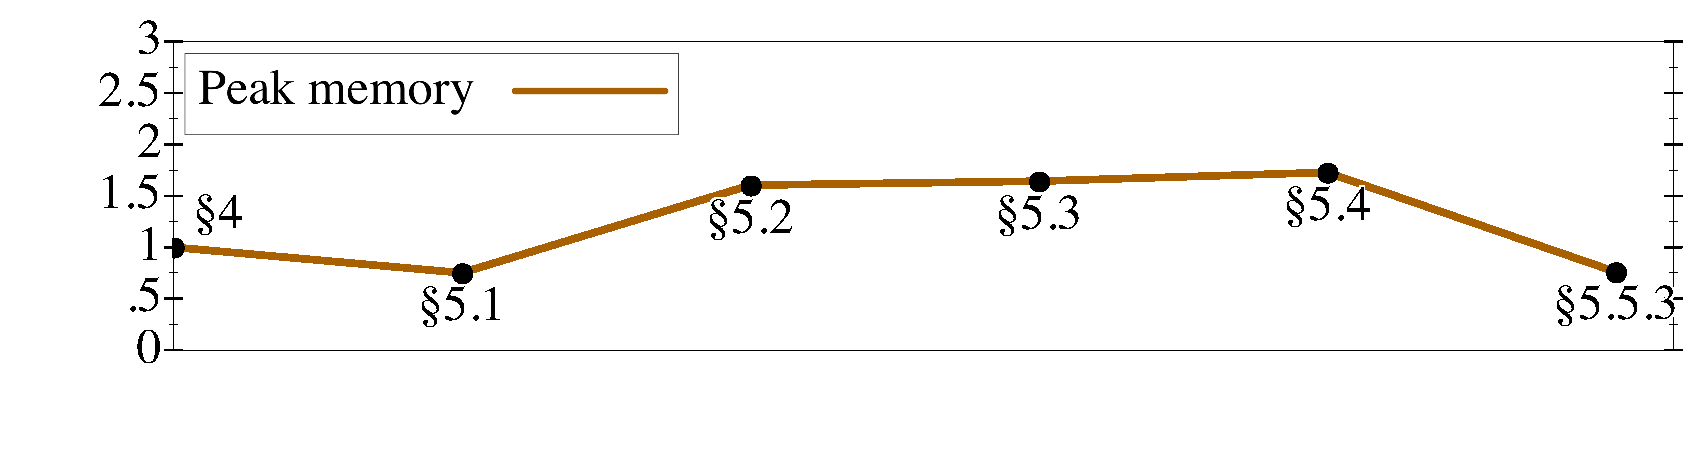
\includegraphics[width=3.2in]{church-relative-space.ps}
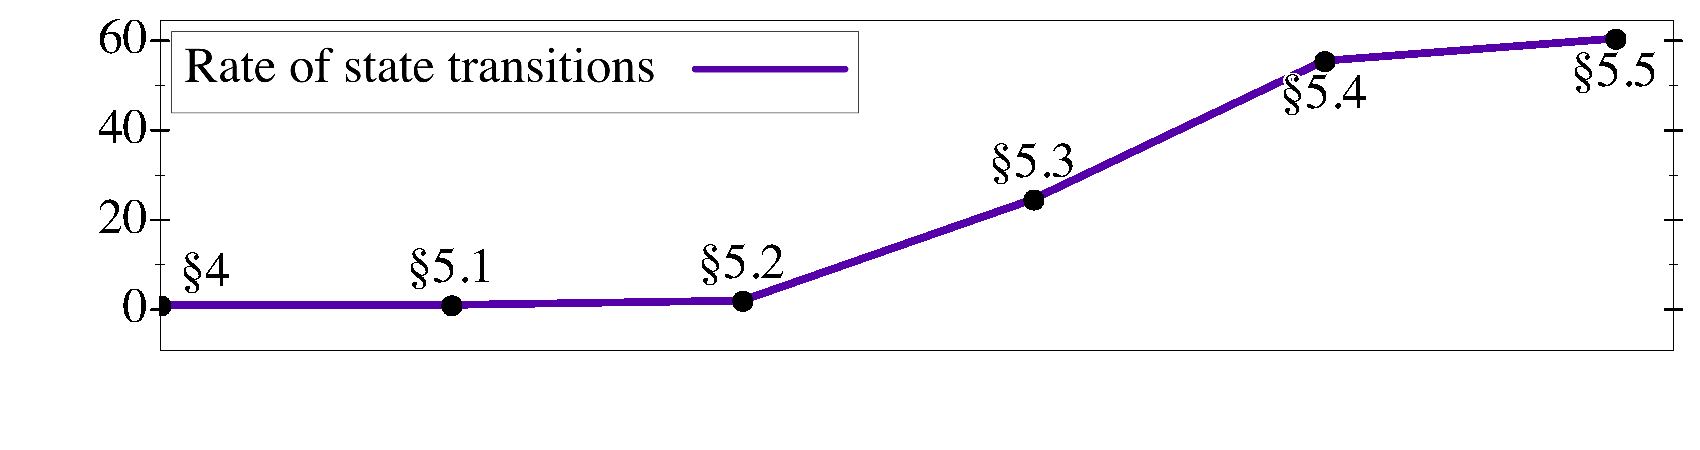
\includegraphics[width=3.2in]{church-relative-speed.ps}
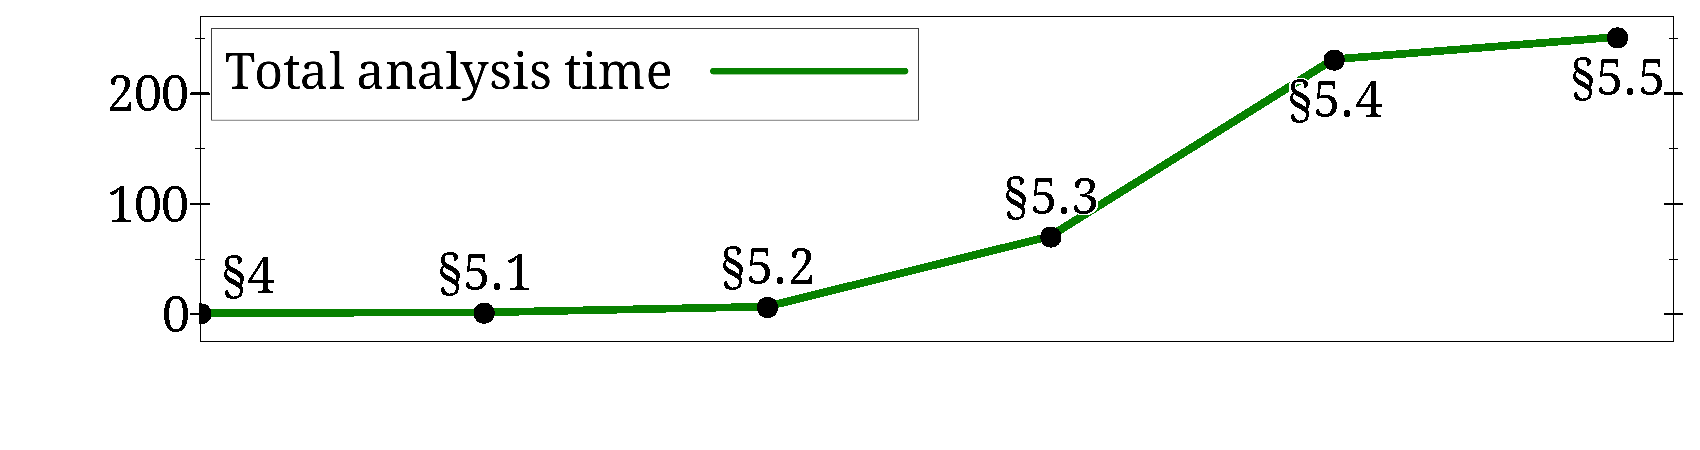
\includegraphics[width=3.2in]{church-relative-time.ps}
\vspace{-1.5em}
\end{center}
\caption{Relative improvements over the baseline analyzer for the
  \Church{} benchmark in terms of peak memory usage, the rate of state
  transitions, and total analysis time. Each point is marked with the
  section that introduces the optimization.}
\label{fig:churchtime}
\end{figure}


This paper is organized in two halfs: in the first, we start with a
quick review of the AAM approach to develop an analysis framework and
then apply our step-by-step optimization techniques in the simplified
setting of a core functional language.  This allows us to explicate
the optimizations with a minimal amount of inessential technical
overhead.  In the second half, we scale this approach up to an
analyzer for a realistic untyped, higher-order imperative language
with a number of interesting features.

At each step during the initial development, we evaluate the
implementation on a benchmark from Vardoulakis and
Shivers~\cite{dvanhorn:Vardoulakis2011CFA2} that tests distributivity
of multiplication over addition on Church numerals.
%% \footnote{It is
%%   written here using Scheme notation and makes use of the shorthands:
%% %
%% \begin{alltt}
%%    (define (((f x) y) z) ...) \(\equiv\)
%%
%%    (define f (\(\lambda\) (x) (\(\lambda\) (y) (\(\lambda\) (z) ...))))
%% \end{alltt}
%%
%% \begin{alltt}
%%    \church{n} \(\equiv\) (\(\lambda\) (s) (\(\lambda\) (z) (s\(\subscript1\) (s\(\subscript2\) ... (s\(\subscript{n}\) z)))))
%% \end{alltt}}
The example, while small, is informative:
\begin{enumerate}
\item it can be written in most modern programming languages,
%
\item it was designed to stress an analyzer's ability to deal with
  complicated environment and control structure arising from the use
  of higher-order functions to encode arithmetic, and
%
\item it proves to be the \emph{least} improved benchmark of the
  complete suite considered in section~\ref{sec:eval}, and thus it
  serves as a good sanity check and lower-bound for each of the
  optimization techniques considered.
\end{enumerate}

We start, in section~\ref{sec:aam}, by developing an abstract
interpreter according to the AAM approach.  Without further
abstraction, the analysis is exponential due to per-state store
variance and thus cannot analyze the example in a reasonable amount of
time.  In section~\ref{sec:baseline}, we perform a further abstraction
by widening the store.  The resulting analyzer sacrifices precision
for speed and is able to analyze the example in about 1 minute.  This
step is described by Van Horn and Might~\cite[\S
  3.5--6]{dvanhorn:VanHorn2012Systematic} and is necessary to make
even small examples feasible.  We therefore take the widened
interpreter as the baseline for our evaluation.

Section~\ref{sec:opt} gives a series of simple abstractions and
implementation techniques that, in total, speed up the analysis by
nearly a factor of 500, dropping the analysis time to a fraction of a
second.  Figure~\ref{fig:churchtime} shows the step-wise improvement
of the analysis time for this example.

%% \newcommand{\church}[1]{\(\ulcorner{\tt #1}\urcorner\)}
%% \begin{figure}
%% \hrule
%% \vspace{2mm}
%% \begin{alltt}
%% (define (zero? n) ((n (\(\lambda\) (zx) #f)) #t))
%% (define (((mult m1) m2) mf) (m2 (m1 mf)))
%% (define ((((plus p1) p2) pf) x)
%%   ((p1 pf) ((p2 pf) x)))

%% (define (((pred n) rf) rx)
%%   (((n (\(\lambda\) (g) (\(\lambda\) (h) (h (g rf)))))
%%     (\(\lambda\) (ignored) rx))
%%    (\(\lambda\) (id) id)))

%% (define ((church=? e1) e2)
%%   (if (zero? e1) (zero? e2)
%%       (if (zero? e2) #f
%%           ((church=? (pred e1)) (pred e2)))))

%% ;; multiplication distributes over addition
%% ((church=? ((mult \church2) ((plus \church1) \church3)))
%%  ((plus ((mult \church2) \church1)) ((mult \church2) \church3)))
%% \end{alltt}
%% \caption{Church-numeral calculation}
%% \label{fig:church}
%% \end{figure}

\begin{figure}[t]
%% \hrule
%% \vspace{2mm}
%% \begin{alltt}
%% (define (id x) x)
%% (define (f n)
%%   (if (<= n 1) 1 (* n (f (- n 1)))))
%% (define (g n)
%%   (if (<= n 1) 1 (+ (* n n) (g (- n 1)))))
%% (print (+ ((id f) 3) ((id g) 4)))
%% \end{alltt}
%% \hrule
\begin{center}
\begin{tabular}{ccc}
\raisebox{1ex-\height}{
\includegraphics[height=3.5in]{introspective-base.pdf}}
&
\raisebox{1ex-\height}{
\includegraphics[height=3.5in]{introspective-lazy.pdf}}
&
\raisebox{1ex-\height}{
\includegraphics[height=3in]{introspective-lazyc.pdf}}
\\
(a) Baseline
&
(b) Lazy
&
(c) Compiled (\& lazy)
\end{tabular}
\end{center}
\caption{Example state graphs for the program above.  Part (a) shows
  the result of the baseline analyzer.  It has long ``corridor''
  transitions and ``diamond'' subgraphs that fan-out from
  nondeterminism and fan-in from joins.  Part (b) shows the result of
  performing nondeterminism lazily and thus avoids many of the diamond
  subgraphs.  Part (c) shows the result of abstract compilation that
  removes intepretive overhead in the form of intermediate states,
  thus minimizing the corridor transitions.  The end result is a more
  compact abstraction of the program that can be generated faster.}
\label{fig:state-graphs}
\end{figure}

The AAM approach, in essence, does the following: it takes a
machine-based view of computation and turns it into a \emph{finitary
  approximation} by bounding the size of the store.  With a limited
address space, the store must map addresses to \emph{sets} of values.
Store updates are interpreted as joins, and store dereferences are
interpreted by non-deterministic choice of an element from a set.  The
result of analyzing a program is a finite directed graph where nodes
in the graph are (abstract) machine states and edges denote machine
transitions between states.

The techniques we propose for optimizing analysis fall into the
following categories:
\begin{enumerate}
\item generate fewer states by avoiding the eager exploration of
  non-deterministic choices that will later collapse into a single
  join point.  We accomplish this by applying lazy evaluation
  techniques so that non-determinism is evaluated \emph{by need}.

\item generate fewer states by avoiding unnecessary, intermediate
  states of a computation.  We accomplish this by applying compilation
  techniques from functional languages to avoid interpretive overhead
  in the machine transition system.

\item generate states faster.  We accomplish this by better algorithm
  design in the fixed-point computation we use to generate state graphs.
\end{enumerate}
Figure~\ref{fig:state-graphs} shows the effect of (1) and (2) for a
small example due to Earl, et
al.~\cite{dvanhorn:Earl2012Introspective}.
By generating significantly fewer states at a significantly faster
rate, we are able to achieve large performance improvements in terms
of both time and space.

Section~\ref{sec:eval} describes the evaluation of each optimiztion
technique applied to an implementation supporting a more realistic set
of features, including mutation, first-class control, compound data, a
full numeric tower and many more forms of primitive data and
operations.
%
We evaluate this implementation against a set of benchmark programs
drawn from the literature.
%
For all benchmarks, the optimized analyzer outperforms the baseline
by at least a factor of
% 475
two to
% 4,382
three orders of magnitude.

Section~\ref{sec:related} relates this work to the literature and
section~\ref{sec:conclusion} concludes.

%\newpage
\section{An abstract$^{\text 2}$ machine for ISWIM}
\label{sec:aam}


ISWIM is a family of programming languages parameterized by a set of
base values and operations.  To make things concrete, we consider a
member of the ISWIM family with integers, booleans, and a few
operations.

\begin{figure}
\[
\begin{array}{l@{\qquad}rcl}
\text{Expressions} & \mathit{e} &=& \svar[^\mlab]\mvar\\
&&|& \slit[^\mlab]\mlit\\
&&|& \slam[^\mlab]\mvar\mexp\\
&&|& \sapp[^\mlab]\mexp\mexp \\
&&|& \sif[^\mlab]\mexp\mexp\mexp \\
\text{Variables}&\mvar &=& \syntax{x}\ |\ \syntax{y}\ |\ \dots\\
\text{Literals}&\mlit &=& \mnum\ |\ \mbln\ |\ \mop\\
\text{Integers}&\mnum &=& \syntax{0}\ |\ \syntax{1}\ |\ \syntax{-1}\ |\ \dots\\
\text{Booleans}&\mbln &=& \strue\ |\ \sfalse\\
\text{Operations}&\mop &=& \syntax{zero?}\ |\ \syntax{add1}\ |\ \syntax{sub1}\ |\ \dots
\end{array}
\]
\caption{Syntax of ISWIM}
\label{fig:syntax}
\end{figure}

Figure~\ref{fig:syntax} defines the (abstract) syntax of ISWIM.
Figure~\ref{fig:aam} defines the semantics of ISWIM as a machine
model.  Evaluation is defined as the set of states reachable by the
reflexive, transitive closure of the machine transition relation.  The
machine is a very slight variation on a standard abstract machine for
ISWIM in ``eval, continue, apply''
form~\cite{dvanhorn:Danvy:DSc}.  It can be
systematically derived from a definitional interpreter through a
continuation-passing style transformation and defunctionalization, or
from a structural operational semantics using the refocusing
construction of Danvy and
Nielsen~\cite{dvanhorn:Danvy-Nielsen:RS-04-26}.

Compared with the standard machine semantics, this definition is
different in the following ways:
\begin{itemize}
\item the store maps addresses to \emph{sets} of values,
\item continuations are heap-allocated,
\item there are ``contour values'' (written $\mcntr$) and syntax
  labels ($\mlab$) threaded through the computation, and
\item the machine is implicitly parameterized by the functions
  $\mathit{push}$, $\mathit{bind}$, $\interpdelta$ and $\sqcup$.
\end{itemize}

\begin{figure}
\begin{gather*}
\begin{align*}
\mathit{eval}(\mexp) &= \{ \mstate\ |\ \ev[^{\mtcntr}]{\mexp,\varnothing,\varnothing,\kmt} \multimachstep \mstate \} \text{ where }
\end{align*}
\\[2mm]
\begin{array}{@{}r@{\ }c@{\ }l@{}}
%% EVAL
\ev{\svar\mvar,\menv,\msto,\mkont} &\machstep&
\co{\mkont,\mval,\msto}
\text{ where }\mval \in \msto(\menv(\mvar))
\\
\ev{\slit\mlit,\menv,\msto,\mkont} &\machstep&
\co{\mkont,\mlit,\msto}
\\
\ev{\slam\mvar\mexp,\menv,\msto,\mkont} &\machstep&
\co{\mkont,\clos{\mvar,\mexp,\menv},\msto}
\\
\ev[^\mcntr]{\sapp[^\mlab]{\mexpi0}{\mexpi1},\menv,\msto,\mkont} &\machstep&
\ev[^\mcntr]{\mexpi{0},\menv,\msto',\kar[_\mlab^\mcntr]{\mexpi{1},\menv,\maddr}}
\\
&&
\text{ where }\maddr,\msto' = \mathit{push}^\mcntr_\mlab(\msto,\mkont)
\\
\ev[^\mcntr]{\sif[^\mlab]{\mexpi0}{\mexpi1}{\mexpi2},\menv,\msto,\mkont} &\machstep&
\ev[^\mcntr]{\mexpi0,\menv,\msto',\kif[^\mcntr]{\mexpi1,\mexpi2,\menv,\maddr}}
\\
&&
\text{ where }\maddr,\msto' = \mathit{push}_\mlab^\mcntr(\msto,\mkont)
\\[2mm]
%% CONTINUE
\co{\kmt,\mval,\msto} &\machstep&
\ans{\msto,\mval}
\\
\co{\kar[^\mcntr_\mlab]{\mexp,\menv,\maddr},\mval,\msto} & \machstep&
\ev[^\mcntr]{\mexp,\menv,\msto,\kfn[^\mcntr_\mlab]{\mval,\maddr}}
\\
\co{\kfn[^\mcntr_\mlab]{{\mvalx{u}},\maddr},\mval,\msto} & \machstep&
\ap[^\mcntr_\mlab]{\mvalx{u},\mval,\mkont,\msto}
\text{ where }\mkont \in \msto(\maddr)
\\
\co{\kif[^\mcntr]{\mexpi0,\mexpi1,\menv,\maddr},\strue,\msto} & \machstep&
\ev[^\mcntr]{\mexpi0,\menv,\msto,\mkont}
\text{ where }\mkont\in\msto(\maddr)
\\
\co{\kif[^\mcntr]{\mexpi0,\mexpi1,\menv,\maddr},\sfalse,\msto} & \machstep&
\ev[^\mcntr]{\mexpi1,\menv,\msto,\mkont}
\text{ where }\mkont\in\msto(\maddr)
\\[2mm]
%% APPLY
\ap[^\mcntr_\mlab]{\clos{\mvar,\mexp,\menv},\mval,\msto,\mkont} & \machstep&
\ev[^{\mcntr'}\!]{\mexp,\menv',\msto',\mkont}
\\
\multicolumn{3}{r@{}}{
\text{ where }\menv',\msto',\mcntr' = \mathit{bind\,}^{ \mcntr}_\mlab(\menv,\msto,\mvar,\mval)}
\\
\ap[^\mcntr_\mlab]{\mop,\mval,\msto,\mkont} & \machstep&
\co{\mkont,\mval',\msto}
\text{ where } \mval'\in\interpdelta(\mop,\mval)
\end{array}
\end{gather*}
\caption{Abstract abstract machine for ISWIM}
\label{fig:aam}
\end{figure}


\paragraph{Concrete interpretation} can be characterized by setting the implicit
parameters of the relation given in Figure~\ref{fig:aam} as follows:
\begin{align*}
\mathit{push}_\mlab^\mcntr(\msto,\mkont) &= \maddr,\msto\sqcup[\maddr\mapsto\{\mkont\}]
\mbox{ where }\maddr \notin\msto
\\
\mathit{bind}(\menv,\msto,\mvar,\mval) &= \menv[\mvar\mapsto\maddr],\msto\sqcup[\maddr\mapsto\{\mval\}]
\mbox{ where }\maddr \notin\msto
\end{align*}
The resulting relation is non-deterministic in its choice of
addresses, however it must always choose a fresh address when
allocating a continuation or variable binding.  If we consider machine
states equivalent up to consistent renaming, this relation defines
a deterministic machine.  (The relation is really a function.)


\paragraph{Abstract interpretation} can be characterized by setting the implicit
parameters just as above, but dropping the $\maddr \not\in \msto$
condition.  This family of interpreters is also non-deterministic in
choices of addresses, but it is free to choose addresses that are
already in use.  Consequently, the machines may be non-deterministic
when multiple values reside in a store location.

It is important to recognize from this definition that \emph{any}
allocation strategy is an abstract
interpretation~\cite{MIGHTANDMANOLIOS}.  In particular, concrete
interpretation is a kind of abstract interpretation.  So is an
interpretation that allocates a single cell into which all bindings
and continuations are stored.  On the one hand is an abstract
interpretation that is non-computable and gives only the ground truth
of a programs behavior; on the other is an abstract interpretation
that is easy to compute but gives little information.  Useful program
analyses lay somewhere in between and can be characterized by their
choice of address representation and allocation strategy.

%% We now have a framework for describing program analysis for the ISWIM
%% family of languages, whereby approximation of both control and
%% environment structure is regulated by the heap and allocation
%% policies.

Uniform \(k\)-CFA is one such analysis.

\paragraph{Uniform \(k\)-CFA} can be characterized by the following allocation
strategy:

\begin{align*}
\mathit{push}_\mlab^\mcntr(\msto,\mkont) &=
  \mlab\mcntr,\msto\sqcup[\mlab\mcntr\mapsto\{\mkont\}] \\
\mathit{bind}^\mcntr_\mlab(\menv,\msto,\mvar,\mval) &= \menv[\mvar \mapsto \maddr],
                                           \msto\sqcup[\maddr \mapsto
                                             \{ \mval\}],
                                           \mcntr' \\
\mbox{where } \mcntr' &= \lfloor\mlab\mcntr\rfloor_k \\
              \maddr &= x\mcntr' \\
%%              \lfloor \mtcntr \rfloor_k &= \mtcntr \\
              \lfloor \mcntr \rfloor_0 &= \mtcntr \\
              \lfloor \mlab\mcntr \rfloor_{k+1} &= \mlab\lfloor \mcntr\rfloor_k
\end{align*}
$\sqcup$ on stores is a point-wise lifting of $\sqcup$: $\msto \sqcup \msto' = \lambda \maddr. \msto(\maddr) \sqcup \msto'(\maddr)$.
For the duration of this paper, since our example abstract value space
has no interesting ordering, $\sqcup$ can be read as $\cup$.
\paragraph{Primitives}

\begin{align*}
\mnum+1 &\in \interpdelta(\saddone,\mnum) &
\mnum-1 &\in \interpdelta(\ssubone,\mnum)\\
\strue &\in \interpdelta(\szerohuh,\szero) &
\sfalse &\in \interpdelta(\szerohuh,\mnum)\text{ if }\mnum\neq \szero\\
\end{align*}

\begin{align*}
\sNum &\in \hat\interpdelta(\saddone,\mnum) &
\sNum &\in \hat\interpdelta(\ssubone,\mnum)\\
\strue &\in \hat\interpdelta(\szerohuh,\sNum) &
\sfalse &\in \hat\interpdelta(\szerohuh,\sNum)\\
\strue &\in \hat\interpdelta(\szerohuh,\szero) &
\sfalse &\in \hat\interpdelta(\szerohuh,\mnum)\text{ if }\mnum\neq \szero\\
\end{align*}

%% \begin{figure}
%% \begin{alltt}
%%   ;; State \(\to\) \(\Set(\)State\()\)
%%   (define (step \(\mstate\))
%%     (match \(\mstate\)
%%       [(ev \(\mexp\) \(\rho\) \(\msto\) \(\mkont\))
%%        (match \(\mexp\)
%%          [(var\(\superscript\mlab\) \(\mvar\))
%%           (for/set ((\(\mval\) (lookup \(\rho\) \(\msto\) \(\mvar\))))
%%             (co \(\msto\) \(\mkont\) \(\mval\)))]
%%          [(lit\(\superscript\mlab\) \(\mlit\)) (set (co \(\msto\) \(\mkont\) \(\mlit\)))]
%%          [(lam\(\superscript\mlab\) \(\mvar\) \(\mexp\)) (set (co \(\msto\) \(\mkont\) (clos \(\mvar\) \(\mexp\) \(\rho\))))]
%%          [(app\(\superscript\mlab\) \(\mexp\subscript0\) \(\mexp\subscript1\))
%%           (define-values (\(\msto'\) \(\maddr\)) (push \(\mstate\)))
%%           (set (ev \(\mexp\subscript0\) \(\rho\) \(\msto'\) (ar \(\mexp\subscript1\) \(\rho\) \(\maddr\))))]
%%          [(ife\(\superscript\mlab\) \(\mexp\subscript0\) \(\mexp\subscript1\) \(\mexp\subscript2\))
%%           (define-values (\(\msto'\) \(\maddr\)) (push \(\mstate\)))
%%           (set (ev \(\mexp\subscript0\) \(\rho\) \(\msto'\) (ifk \(\mexp\subscript1\) \(\mexp\subscript2\) \(\rho\) \(\maddr\))))])]
%%       [(co \(\msto\) \(\mkont\) \(\mval\))
%%        (match \(\mkont\)
%%          ['mt (set (ans \(\msto\) \(\mval\)))]
%%          [(ar\(\superscript\mlab\) \(\mexp\) \(\rho\)) (set (ev \(\mexp\) \(\rho\) \(\msto\) (fn \(\mval\) l)))]
%%          [(fn\(\superscript\mlab\) \(\mval'\))
%%           (for/set ((\(\mkont\) (get-cont \(\msto\) l)))
%%             (ap \(\msto\) \(\mval'\) \(\mval\) \(\mkont\)))]
%%          [(fi\(\superscript\mlab\) c a \(\rho\))
%%           (for/set ((k (get-cont \(\msto\) l)))
%%             (ev (if v c \(\maddr\)) \(\rho\) \(\msto\) \(\mkont\)))])]
%%       [(ap \(\msto\) fun \(\maddr\) \(\mkont\))
%%        (match fun
%%          [(clos l \(\mvar\) \(\mexp\) \(\rho\))
%%           (define-values (\(\rho'\) \(\msto'\)) (bind \(\mstate\)))
%%           (set (ev \(\msto'\) \(\mexp\) \(\rho'\) \(\mkont\)))]
%%          [(op \(\mop\))
%%           (for*/set ((\(\mkont\) (get-cont \(\msto\) l))
%%                      (\(\mval\) (\(\interpdelta\) \(\mop\) \(\mval\))))
%%             (co \(\msto\) \(\mkont\) \(\mval\)))]
%%          [_ (set)]))]))
%% \end{alltt}
%% \caption{Implementation of machine transition relation.}
%% \end{figure}

\section{Reduction semantics to baseline analyzer}
\label{sec:baseline}

The uniform $k$-CFA allocation strategy would make $eval$ in figure
\ref{fig:aam} a computable abstraction of reachable states, but not an
efficient one. This is not the strategy that AAM, nor we, recommend. Through
this and the following section, we will explain a succession of approximations
to reach the baseline analysis.  We'll compare performance at each stage to
identify the criticality of each optimization. 
%
We ground this journey by first formulating the analysis in terms of a classic
fixed-point computation.


\subsection{Static analysis as fixed-point computation}
\label{sec:fixpoint}

Conceptually, the AAM approach calls for computing an analysis as a graph
exploration: (1) start with an initial state, and (2) compute the transitive
closure of the transition relation starting from that state.

We can cast this exploration process in terms of a fixed-point calculation.
%
Given the initial state $\varsigma_0$ and the transition relation $\machstep$,
we define the global transfer function:
\begin{equation*}
 F_{\varsigma_0} : \mathcal{P}(\mathit{State}) \to \mathcal{P}(\mathit{State})
 \text.
\end{equation*}
Internally, this global transfer function computes the successors of all supplied states, and then includes the inital state:
\begin{equation*}
  F_{\varsigma_0}(S) = \{ \varsigma_0 \} \cup \{ \varsigma' \mathrel{|} \varsigma \in S \text{ and } \varsigma \machstep \varsigma' \}\text. 
\end{equation*}
Then, the evaluator for the analysis computes the least fixed point of the global transfer function:
\begin{equation*}
 \eval(e) = \mathrm{lfp}(F_{\varsigma_0})\text{,}
\end{equation*}
where $\varsigma_0 = \ev[^\mtcntr]{e, \varnothing, \varnothing, \kmt}$.


To conduct this naive exploration on the \Church{} example would require
considerable time.  Even though the state space is finite, it is exponential in
the size of the program.  Even with $k = 0$, there are exponentially many
stores in the AAM framework.

In the next subsection, we'll fix this with a widening and reach polynomial
(albeit of a high degree) complexity.
%
This widening effictively lifts the store out of individual states to create
a single, global shared store for all.


\subsection{Store widening}
\label{sec:storewiden}

A common technique to accelerate convergence in flow analyses is to share a
common, global store.
%
To retain soundness, this store grows monotonically.
%
Formally, we can cast this optimization as a second abstraction or as the
application of a widening operator during the fixed-point iteration.
%
In the ISWIM language, such a widening makes 0CFA quartic in the size of the
program.
%
Thus, in one step, complexity drops from intractable exponentiality to merely
daunting polynomiality.

Since we can cast this optimization as a widening, there is no need to change
the transition relation itself.
%
Rather, what changes is the structure of the fixed-point iteration.
%
In each pass, the algorithm will collect all newly produced stores and join
them together.
%
Then, before each transition, it will install this joined store into current
state.

To describe this process, we'll refactor the transition relation so that it operates on
a pair of a set of contexts ($C$) and a store ($\sigma$).
%
A context includes all non-store components, \emph{e.g.}, the expression, the environment and the stack.
%
The refactored relation, $\widehat{\machstep}$, becomes:
%
\begin{align*}
(C, \msto) &\mathrel{\widehat{\machstep}} (C', \msto') \\
\mbox{where } C' &= \{c' \mid wn(c, \msto) \mathrel{\machstep} wn(c, \msto^c), c \in C\} \\
              \msto' &= \bigsqcup\; \{\msto^c \mid wn(c,\msto)\mathrel{\machstep} wn(c', \msto^c), c \in C\} \\
wn(\ev{\mexp, \menv, \mkont}, \msto) &= \ev{\mexp, \menv, \msto, \mkont} \\
wn(\co{\mval, \mkont}, \msto) &= \co{\mval, \msto, \mkont} \\
wn(\ap{\mvalx{u}, \mval, \mkont}, \msto) &= \ap{\mvalx{u}, \mval, \msto, \mkont} \\
wn(\ans{\mval}, \msto) &= \ans{\msto, \mval}
\end{align*}
%
In effect, the new store is computed as the least upper bound of all subsequent stores.


\subsection{Store-allocated results}
\label{sec:baselineeval}

The final approximation we make to get to our baseline analysis is
store-allocating results of application sub-expressions. The semantics
of the previous section is where AAM leaves off. However, notice that
the $\kfn{}$ continuation stores a value - this makes the space of
continuations quadratic rather than linear in 0-CFA. A linear space
drops the complexity to cubic.

To achieve this, we instead allocate an address for the value position
when we create the continuation.  This address and the tail address
are both determined by the label of the application point, so the
space becomes linear and the overall complexity drops to cubic. Note
that this is a critical abstraction in languages with n-ary functions,
since otherwise the continuation space becomes ${\mathcal O}(n^n)$!
This amount of distinction between continuations is unnecessary
in practice.

The important rules that change are the following, specialized to 0-CFA:

\newcommand{\ext}[3]{#1\sqcup[#2\mapsto#3]}
%\newcommand{\ext}[3]{ext(#1,#2,#3)}

\begin{align*}
%ext(\msto, \maddr, s) &= \msto \sqcup [\maddr \mapsto s] \\
\ev{\sapp[^\mlab]{\mexpi0}{\mexpi1},\menv,\msto,\mkont} &\machstep
\ev{\mexpi{0},\menv,\ext{\msto}{\mlab}{\{\mkont\}},\kar{\mexpi{1},\mlab}}
\\
\co{\kar{\mexp,\menv,\mlab},\mval,\msto} & \machstep
\ev{\mexp,\menv,\ext{\msto}{\mlab^f}{\{\mval\}},\kfn{\mlab^f,\mlab}}
\\
\co{\kfn{\mlab^f,\mlab},\mval,\msto} & \machstep
\ap[_\mlab]{\mvalx{u},\mlab^a,\mkont,\ext{\msto}{\mlab^a}{\{\mval\}}}
\\
\text{ where } &\mkont \in \msto(\maddr), \mvalx{u} \in \msto(\maddr^f)
\\
\ap[_\mlab]{\clos{\mvar,\mexp,\menv},\mlab^a, \msto,\mkont} & \machstep
\ev{\mexp,\menv[\mvar\mapsto\mvar],\ext{\msto}{\mvar}{\msto(\mlab^a)},\mkont}
\\
\ap[_\mlab]{\mop,\mlab^a,\msto,\mkont} & \machstep
\co{\mkont,\mval',\msto}
\\
\text{ where }& \mval'\in \{\interpdelta(\mop,\mval) \mid \mval \in \msto(\mlab^a)\}
\end{align*}

This extra store-allocation is effectively naming all intermediate
results, and thus the precision aligns with an analysis specialized to
ANF. We can also play a representation trick in 0-CFA and remove
$\menv$. In monovariant analyses, variables map to themselves, meaning
$\menv$ is effectively the identity function. That degeneration, in
turn, allows us to discard it from the analysis.

% Wide Store: cpu time: 551571 real time: 571319 gc time: 4003

\section{Implementation techniques}
\label{sec:opt}

We discuss a succession of techniques for increasing performance by
decreasing the interpretive overhead of abstract interpretation. They
come in two flavors: decreasing the size of the state space with domain-specific knowledge [DSK], and
decreasing the amount of intermediate data structures [Eng](ineering).

\begin{enumerate}
 \item{[DSK] lazy non-determinism: quotient by sets of values}
 \item{[DSK] abstract compilation: eliminate {\tt ev} states}
 \item{[Eng] store deltas: operate on store changes rather than whole stores}
 \item{[DSK/Eng] timestamp: represent the store as a global, mutable
   hash and determine a state's store by the number of changes made to
   the global store at the time of visiting}
 \item{[Eng] preallocation: represent the global store as a global, mutable vector}
 \item{[DSK] uniform literal approximation: coarsely abstract literal data}
\end{enumerate}

Some techniques preserve the precision of the underlying analysis, and
others do not. We will discuss the design decisions behind the
precision-lossy techniques.  Each technique requires minimal changes
to the reduction relation, and each improves performance by
integer factors.

\subsection{Lazy non-determinism}

A shortcoming of the AAM approach is that much of the non-determinism
is spurious. For example, in a function application, {\tt (f x y)},
where all variables have been joined with multiple values, each
variable reference transitions to as many new states as there are
values, only to be joined back together in their respective
application positions. We would see transitions of the following
shape:
\begin{center}
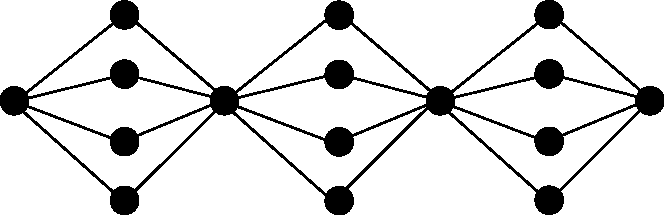
\includegraphics[scale=0.3]{fanout.pdf}
\end{center}
For this reason, we {\it delay} the non-determinism
until it is needed in {\it strict contexts} (such as the guard for an
{\tt if} a called procedure, or a numerical primitive application). We instead get transitions of this shape:
\begin{center}

\includegraphics[scale=0.3]{lazy.pdf}
\end{center}

This does not change the concrete semantics of the language. It is an
abstraction of the otherwise several states the original
non-deterministic semantics steps to. We say the abstraction is
\emph{lazy} because it delays dereferencing an address until its
contents are \emph{needed} as values in the semantics. It does not
change the execution order that leads to the values that are stored in
the address.

We introduce a new kind of value, $\saddr{\maddr}$, that represents a
delayed lookup of $\maddr$. This acts to quotient the state space by
the values at the delayed address. The following rules highlight the
changes to the semantics:

\begin{align*}
force &: \Store \times \Addr \to \Set(\Value) \\
force(\msto,\saddr\maddralt) &= \msto(\maddralt)\\
force(\msto,\mval) &= \{\mval\} \\
ext(\msto, \maddr, \mval) &= \msto \sqcup[\maddr \mapsto force(\msto, \mval)] \\
\ev{\svar{\mvar},\menv,\mkont,\msto} &\machstep\;
\co{\mkont,\saddr{\menv(\mvar)},\msto} \\
\co{\kar[^\mcntr_\mlab]{\mexp,\menv,\maddr},\mval,\msto}
&\machstep\;
\ev[^\mcntr]{\mexp,\menv,ext(\msto, \maddr^f,\mval),\kfn[^\mcntr_\mlab]{\maddr^f,\maddr}} \\
bind^\mcntr_\mlab(\menv,\msto,\mvar,\mval) &= \menv[\mvar \mapsto
  \maddr], ext(\msto,\maddr, \mval), \mcntr' \\
\mbox{where } \mcntr' &= \lfloor\mlab\mcntr\rfloor_k \\
              \maddr &= \mvar\mcntr'
\end{align*}

\paragraph{Lose precision; simplify implementation}
This semantics introduces a subtle precision difference over the
baseline. Consider a configuration where a reference to a variable and
a binding of a variable will happen in one step. With laziness, the
reference will mean the original binding(s) of the variable or the new
one, because the actual store lookup is delayed one step
(i.e. laziness is administrative). Without laziness, the reference
will fan out to all the bindings of the variable before the new
binding happens and thus might have an observable precision
difference.

\paragraph{Regain precision; complicate implementation}
The administrative nature of laziness means that we could remove the
loss in precision by duplicating the reduction relation to specialize
variable lookup. This works since in the semantics of ISWIM with
store-allocated results consumes the value component of states in one
step. This is not the case for semantics that replicate the value
component across reductions, say for popping off exception handler
frames. Further convolution is needed to remove the administrative
nature of laziness in these semantics. Due to the increase of
conceptual complexity for negligable benefit, we decided against this
approach.

\paragraph{Our choice: option 1}
The configurations that lead to precision loss happen too rarely to
warrant the significant increase in time and memory needed for this
eager non-determinism. Indeed, were the variable reference a step
later and another binding not made in that step, the results of the
two approaches are the same.

% Lazy:  cpu time: 32481 real time: 32881 gc time: 547

\subsection{Abstract compilation}

The laziness optimization saved time by doing the same amount of
reasoning as before but in fewer transitions. We can exploit the same
idea - same reasoning, fewer transitions - with abstract
compilation. Abstract compilation is \emph{precision-preserving} and
transforms complex expressions whose \emph{abstract} evaluation is
deterministic into ``abstract bytecodes.''  The abstract interpreter
then does in one transition what previously took many. Abstract
compilation eliminates unnecessary allocation, deallocation and
branching.

The essence of the compilation effect can be seen by considering an
example such as
\[
\sapp{\sapp{\sapp\mvar{\mexp_1}}{\mexp_2}}{\mexp_3}
\]
which makes the following transitions:
\begin{align}
& \ev{\sapp{\sapp{\sapp\mvar{\mexp_1}}{\mexp_2}}{\mexp_3},\menv,\mkont,\msto_0}\\
\machstep\; &
\ev{\sapp{\sapp\mvar{\mexp_1}}{\mexp_2},\menv,\kar{\mexp_3,\menv,\maddr_1},\msto_1}
\\
\machstep\; &
\ev{\sapp\mvar{\mexp_1},\menv,\kar{\mexp_2,\menv,\maddr_2},\msto_2}
\\
\machstep\; &
\ev{\mvar, \menv,\kar{\mexp_1,\menv,\maddr_3},\msto_3} % {\mexp_2}
\\
\machstep\; &
\co{\kar{\mexp_1,\menv},\mval,\msto_4} % {\mexp_1}{\mexp_2}
\mbox{ where } \mval \in \msto(\menv(\maddr))
\end{align}

where $\msto_4 = \msto_0 \sqcup \{ [\maddr_1 \mapsto \{ \mkont \}],
[\maddr_2 \mapsto \kar{\mexp_3,\menv,\maddr_1}]
[\maddr_3 \mapsto \kar{\mexp_2,\menv,\maddr_2}]$.

The compilation step converts expressions into functions that expect
the other components of the {\tt ev} state. Its definition in figure
\ref{fig:compile} shows close similarity to the rules for interpreting
    {\tt ev} states. The next step is to change reduction rules that
    create {\tt ev} states to instead call these functions. Figure
    \ref{fig:caam} shows the modified reduction relation.

\begin{figure}
\begin{align*}
\compile{\_} &: \Expr \to \Env \times \Store \times \Kont \to \State \\
\compile{\svar\mvar} &= \lambda(\menv,\msto,\mkont) .\co{\mkont,\saddr{\menv(\mvar)},\msto}
\\
\compile{\slit\mlit} &= \lambda(\menv,\msto,\mkont) .
\co{\mkont,\mlit,\msto}
\\
\compile{\slam\mvar\mexp} &= \lambda(\menv,\msto,\mkont) .
\co{\mkont,\clos{\mvar,\compile\mexp,\menv},\msto}
\\
\compile{\sapp[^\mlab]{\mexpi0}{\mexpi1}} &= \lambda^\mcntr(\menv,\msto,\mkont) .
\compile{\mexpi0}^\mcntr(\menv,\msto',\kar[_\mlab^\mcntr]{\compile{\mexpi1},\menv,\maddr})
\\
&
\text{ where }\maddr,\msto' = \mathit{push}^\mcntr_\mlab(\msto,\mkont)
\\
\compile{\sif[^\mlab]{\mexpi0}{\mexpi1}{\mexpi2}} &= \lambda^\mcntr(\menv,\msto,\mkont) .
\compile{\mexpi0}^\delta(\menv,\msto',\kif[^\mcntr]{\compile{\mexpi1},\compile{\mexpi2},\menv,\maddr})
\\
&\text{ where }\maddr,\msto' = \mathit{push}_\mlab^\mcntr(\msto,\mkont)
\end{align*}
\caption{Abstract compilation}
\label{fig:compile}
\end{figure}

\begin{figure}
\begin{align*}
\mathit{eval}(\mexp) &= \{ \mstate\ |\ \compile{\mexp}(\epsilon,\varnothing,\varnothing,\kmt) \multimachstep \mstate \} \text{ where }
\\[2mm]
%% CONTINUE
\co{\kmt,\mval,\msto} &\machstep
\ans{\msto,\mval}
\\
\co{\kar[^\mcntr_\mlab]{\mcomp,\menv,\maddr},\mval,\msto} & \machstep
\mcomp^\mcntr(\menv,\msto,\kfn[^\mcntr_\mlab]{\mval,\maddr})
\\
\co{\kfn[^\mcntr_\mlab]{{\mvalx{u}},\maddr},\mval,\msto} & \machstep
\ap[^\mcntr_\mlab]{\mval,\mvalx{u},\mkont,\msto}
\text{ where }\mkont \in \msto(\maddr)
\\
\co{\kif[^\mcntr]{\mcompi0,\mcompi1,\menv,\maddr},\strue,\msto} & \machstep
\mcompi0^\mcntr(\menv,\msto,\mkont)
\text{ where }\mkont\in\msto(\maddr)
\\
\co{\kif[^\mcntr]{\mcompi0,\mcompi1,\menv,\maddr},\sfalse,\msto} & \machstep
\mcompi1^\mcntr(\menv,\msto,\mkont)
\text{ where }\mkont\in\msto(\maddr)
\\[2mm]
%% APPLY
\ap[^\mcntr_\mlab]{\clos{\mvar,\mcomp,\menv},\mval,\msto,\mkont} & \machstep
\mcomp^{\mcntr'}(\menv',\msto',\mkont) \\
\text{ where }\menv',\msto',\mcntr' &= \mathit{bind\,}^{ \mcntr}_\mlab(\menv,\msto,\mvar,\mval)
\\
\ap{\mop,\mval,\msto,\mkont} & \machstep
\co{\mkont,\mval',\msto} \\
\text{ where }\mkont &\in\msto(\maddr)
\text{ and } \mval'\in\interpdelta(\mop,\mval)
\end{align*}
\caption{Abstract$^2$ machine for compiled ISWIM}
\label{fig:caam}
\end{figure}

% Compile: cpu time: 255397 real time: 261532 gc time: 2947

% \noindent
% Compile + Lazy: cpu time: 31173 real time: 31642 gc time: 739

%\newpage

\subsection{Locally log-based store deltas}

Every step the analysis makes for the above techniques requires
joining large stores together. Not every step will modify all
addresses of the store, so joining entire stores is wasteful in terms
of memory and time. We can instead log store changes and replay the
change log on the full store after all steps have completed. This uses
far fewer join operations, leading to less overhead, and is \emph{precision preserving}.

We represent changes as $\msdiff \in \StoreDelta = List[\Addr \times
  \Set(\Storeable)]$. Each $\msto\sqcup[\maddr \mapsto \mval{s}]$
instead becomes a log addition
$\cons{\ttuple{\maddr}{\mval{s}}}{\msdiff}$, where $\msdiff$ begins
empty ($\mtlst$) for each step. Applying the changes to the full store
is straightforward:

\begin{align*}
replay &: \StoreDelta \times \Store \to \Store \\
replay(\mtlst, \msto) &= \msto \\
replay(\cons{\ttuple{\maddr}{\mval{s}}}{\msdiff}, \msto) &= replay(\msdiff, \msto\sqcup[\maddr \mapsto \mval{s}])
\end{align*}

The reduction relation does have to change to accommodate this
technique, but only in this regard. The whole store is still given so
that lookups are possible. Example rule:

\begin{align*}
(\ap[^\mcntr_\mlab]{\clos{\mvar,\mexp,\menv},\mval,\mkont},\msto,\msdiff) & \machstep
(\ev[^{\mcntr'}]{\mexp,\menv',\mkont},\msdiff') \\
\text{ where }\menv',\msdiff',\mcntr' &= \mathit{bind\,}^{ \mcntr}_\mlab(\menv,\msto,\msdiff,\mvar,\mval)
\end{align*}
\begin{align*}
bind^{\mcntr}_\mlab(\menv, \msto, \msdiff, \mvar, \mval) &= \menv[\mvar \mapsto \maddr], \cons{\ttuple{\maddr}{force(\msto,\mval)}}{\msdiff}, \mcntr' \\
\text{ where } \mcntr' &= \lfloor \mlab \mcntr\rfloor_k \\
               \maddr &= \mvar\mcntr'
\end{align*}
Compilation changes to additionally take a $\msdiff$ component, so the
above rule's right hand side would instead be $k^{\mcntr'}(\menv',
\msto, \msdiff', \mkont)$ where $k = \compile{e}$ would be in the closure.

We also lift $\machstep$ to accommodate for this asymmetry
in the input and output. For each state that is stepped, we feed the
output changes to the next so that all changes get accumulated:

\begin{align*}
(cs, \msto) &\mathrel{\widehat{\machstep}} (cs\cup cs', replay(\msdiff,\msto)) \\
\mbox{ where } (cs', \msdiff) &= step^*(\varnothing, cs, \mtlst) \\
step^*(S, \varnothing, \msdiff) &= (S, \msdiff) \\
step^*(S, \{c\}\cup cs, \msdiff &= step^*(S\cup cs^*, cs, \msdiff^*) \\
cs^* &= \{c' \mid (c,\msto,\msdiff) \machstep (c',\msdiff^c) \} \\
\msdiff^* &= concat\{\msdiff^c \mid (c, \msto,\msdiff) \machstep (c', \msdiff^c)\}
\end{align*}

Here $concat : \Set(\StoreDelta) \to \StoreDelta$ flattens the lists
of changes to one; order it appends does not matter:
\begin{align*}
concat(\varnothing) &= \mtlst \\
concat(\{\msdiff\}\cup D) &= append(\msdiff, concat(D))
\end{align*}

%% Delta Store +k Compile + Lazy:
%%    cpu time: 668 real time: 686 gc time: 41

\subsection{Timestamping an imperative store}

Thus far, we have made our optimizations in a purely functional
manner. For the next series of optimizations, we need to dip into the
imperative. We can motivate this entire sequence of optimizations by
focusing on the largest bottleneck in the current state-space
exploration algorithm: checking to see if a state has already been
seen. Given two states, checking equality is expensive because the
stores within each are large, and every entry must be checked against
every other. Hashes can sometimes rule out inequality relatively
quickly, but the incidence of collisions and actual equality is
costly.

And, there is a better way. Shivers' original work on k-CFA was
susceptible to the same problem, and he suggested three complementary
optimizations: (1) make the store global; (2) update the store
imperatively; and (3) associate every change in the store with a
version number -- its timestamp. Then, put timestamps in states
where previously there were stores. Given two states, the analysis can
now compare their stores just by comparing their timestamps -- a
constant-time operation.

There is a subtle loss of precision and Shivers' original time-stamp
technique that we can fix. For a given abstract state, all writes to
the global store need to be delayed until the analysis considers all
branches from that abstract state. This avoids cross-branch pollution
which would not otherwise happen, e.g., when one branch writes to
address $\maddr$ and another branch reads from address
$\maddr$. Fortunately, given our conversion to log-based stores this
change is straightforward.

The current state of the state-space search now has six components:

\begin{itemize}
 \item{{\tt $\msto$}, the store}
 \item{{\tt todo}, the workset}
 \item{{\tt seen}, a map from states to the timestamps at which they were last seen}
 \item{{\tt $\msdiff$}, the store changes for the current step}
 \item{{\tt $\msdiff$?}, a boolean tracking whether the stepped state contributed a store change}
 \item{{\tt T}, the timestamp of the store}
\end{itemize}

The new $eval$ calculation is defined in
figure~\ref{fig:imperative}.  To ensure termination, we guard adding
$c$ to {\tt todo} by the following check:
\begin{align*}\msdiff\mbox{{\tt ?}} \vee {\tt seen}(c) \neq {\tt T}\end{align*}
If it succeeds, {\tt todo} gets $c$ and we update {\tt seen} to map $c$ to {\tt T}.

After all steps complete, we apply $\msdiff$ to $\msto$ imperatively
(with {\tt replay!}) and increase {\tt T} as long as there was at
least one change in $\msdiff$. This logic leads to termination if we
know that each $\ttuple{\maddr}{\mval{s}}$ in $\msdiff$ would change
the value of $\maddr$ in the current store. Thus, we also guard
additions to $\msdiff$ so that only updates that would change the
store are permitted. Each time $\msdiff$ is successfully extended, we
set {\tt $\msdiff$?} to true. Before each individual step, we set it
to false.

\begin{figure}
\begin{alltt}
eval(\(e\)) :=
  \(\msto\), todo, seen, T := \(\varnothing\), \(\varnothing\), [], 0
  \(\compile{e}\)(\(\mtcntr, \varnothing, \varnothing, \kmt\))
  while(true):
    if todo = \(\varnothing\): return (keys(seen), \(\msto\))
    else:
      let old := todo
      todo, \(\msdiff\) := \(\varnothing\), \(\mtlst\)
      foreach c \(\in\) old: \(\msdiff\)? := false; c()
      unless \(\msdiff\) = \(\mtlst\): T += 1; replay!(\(\msdiff, \msto\))
\end{alltt}
\caption{Imperative algorithm}
\label{fig:imperative}
\end{figure}

\subsection{Pre-allocating the store}

Internally, the algorithm at this stage uses hash tables to model the store.
%
This is because stores used to be distributed to all states, which
required a compact, dynamic representation.
%
But, such a dynamic structure isn't necessary when we know the
structure of the store in advance: we know all possible entries, and
we know its maximum size.

In a monovariant analysis, the domain of the store is
exactly the set of expressions in the program.
%
If we label each expression with a unique natural, the analysis can
index directly into the store without a hash or a collision.
%
Even for polyvariant analyses, it is possible to compute the maximum
number of addresses and similarly pre-allocate either the spine of the
store or (if memory is no concern) the entire store.

\subsection{Abstracting literal compound data}

Practical issues of performance arise when one chooses the
``obvious,'' or ``natural'' abstraction for compound data. Our running
example will be the classic Boyer benchmark. The detail of note for
the Boyer benchmark is that it has large list literals, the exact
values of which do not matter for many analyses. If we
interpret a list literal of 30 elements (that again have 10 elements
each) as 300 applications of {\tt cons}, and then interpret a function
that traverses the tree, we will end up interpreting that function at
least 300 times, when once or twice would do.

We will first explain the natural abstraction of tuples, and then we
will explain a less precise allocation strategy from uniform $k$-CFA
that we use for large compound data literals that we modified from the
implementation in \citep{dvanhorn:wright-jagannathan-toplas98}.

\subsubsection{Na\"ively}

The uniform way AAM approaches a simple abstraction strategy is to cut
recursion out of the data definition by tying the recursive knot
through the abstract store. For Scheme, the grammar for values looks
like the following:

\newcommand{\alt}{\;\mid\;}
\begin{align*}
\Value &::= \mbox{{\tt \#t}} \alt \mbox{{\tt \#f}} \alt \mbox{{\tt(cons $\Value$ $\Value$)}} \alt \mbox{{\tt '()}} \alt ...
\end{align*}

Upon evaluating a {\tt cons} application, we instead allocate two
addresses $a$ and $d$, join them to the respective values in the
store, and return the flattened {\tt (cons $a$ $d$)} value. Since
these addresses are all distinguished at different syntactic callsites
in the uniform $k$-CFA allocation strategy, and quoted lists are sugar
for a sequence of calls to {\tt cons}, this abstraction explodes the
value space. Analyzing a function that counts the number of atoms in a
literal s-expression would actually interpret that function at least
that number of times (more because of intermediate conses). Indeed,
even in our fastest implementation, this abstraction causes the
analysis of Boyer to be 430 times slower than the approach we will now
describe.

\subsubsection{Less na\"ively and less precisely}

The number of syntactic uses of {\tt cons} versus implicit uses via
literal lists is smaller in typical Scheme programs. We use the above
abstraction for these syntactic uses, but choose to interpret literal
lists as not always sugar for cascading {\tt cons}es. In particular,
if a list literal is ``too big'' (in our case length $>$ 1), we
interpret the list as a circular data structure; the right address
points back to the {\tt cons} itself, and the left address points to
all of the elements of the list. We take this farther and join the
list elements together in with a coarse type-based abstraction. In
effect, large lists or vectors of literal numbers become unbounded
lists/vectors of ``number.'' Heterogeneous data is combined to just
``data,'' rather than a union of ``number'', ``string'', etc. since
primitives are interpreted on every combination of values that flow to
them, and unions lead to more primitive interpretations.

Quotation is special because it cannot introduce function values,
which is important to enhancing our technique's soundness to
conceptual complexity ratio. If we join two values of different type
together, we don't get ``anything,'' which has complex meaning in
higher-order languages (Shivers' escape semantics) and is overly
approximate. We instead get ``any quotable value,'' which has much
simpler semantics.

There are a few steps to consider:
\begin{itemize}
 \item{Define special value lattice elements for compound data domains that can be quoted
       (e.g. {\tt QPair} for $\left\{ ({\tt cons} a_i d_i)\right\}_i$, {\tt QVector} for immutable vectors, etc.)}
 \item{Define a ``larger'' value lattice element for all quotable data, {\tt QData}}
 \item{Interpret {\tt (quote (a ...))} as {\tt (qlist a ...)}, a new primitive function defined in figure \ref{fig:qlist},
       and similar definitions for immutable vectors.}
 \item{Extend the $\interpdelta$ axioms to include conservative
   meaning for these new values (e.g. {\tt (car QData)} = {\tt QData},
   {\tt (add1 QData)} = {\tt Number} and log ``possible type error'')
   and allow them to allocate addresses and change the store}
\end{itemize}

\begin{figure}
\begin{align*}
\interpdelta(\msto, qlist) &= (\mbox{{\tt '()}}, \msto) \\
\interpdelta(\msto, qlist, v ..._+) &= (({\tt cons}\ a\ d), \msto') \\
\qquad \mbox{where } \msto' &= \msto\sqcup[a \mapsto \bigsqcup(v ...)] \\
                            &\qquad \sqcup[d \mapsto \{ \mbox{{\tt '()}}, ({\tt cons}\ a\ d)\}] \\
\bigsqcup(v) &= v \\
\bigsqcup(v, vs ...) &= merge(v, \bigsqcup(vs ...)) \\
merge(v, v) &= v \\
merge(n, m) &= {\tt Number} \\
merge(n, v) &= {\tt QData} \\
merge(({\tt cons}\ a\ d), ({\tt cons}\ a'\ d')) &= {\tt QPair} \\
merge({\tt QPair}, ({\tt cons}\ a\ d)) &= {\tt QPair} \\
merge({\tt QPair}, v) &= {\tt QData} \\
\vdots
\end{align*}
\caption{Quoted list primitive}
\label{fig:qlist}
\end{figure}

\paragraph{Mutable literal data}
The Scheme we model is nonstandard in that it has immutable literal
data (the Scheme benchmarks did not mutate their literal data). To
support mutable literal data, abstract values like {\tt QPair} would
be like regular conses, only point to a preallocated pair of addresses
that hold {\tt QData} as well. This is because conses can be mutated
to hold any value, not just quoted data.

\section{Evaluation}
\label{sec:eval}

We have implemented, optimized, and evaluated \emph{all} of the
machines presented in their JFP paper
\cite{dvanhorn:VanHorn2012Systematic}, with the exception of the
machine for performing pushdown flow analysis.  This includes machines
supporting higher-order functions, state, first-class control,
laziness, and stack inspection.

For each benchmark, we collect analysis times, peak memory usage, and
the rate of states-per-second explored by the analysis for each of the
optimizations discussed in section~\ref{sec:opt}, culmulatively
applied.  The analysis is stopped after consuming 30 minutes of time
or 1 gigabyte of space.  When presenting \emph{relative} numbers, we
use the timeout limits as a lower bound on the actual time required,
thus giving a conservative estimate of improvements.

All benchmarks are calculated as an average of N runs on a [MACHINE
  SPECS].

The benchmarks make use of mutation, first-class control (in the form
of Scheme's {\tt call/cc} operator), compound data such as lists and
vectors, many more primitive forms of data and operations such as
Scheme's numeric tower including exact rationals, complex, and
floating point numbers.

Many benchmarks cause the baseline analyzer to take longer than 30
minutes or to consume more 1 gigabyte of memory, at which point the
analysis is stopped.  This is the case for the largest benchmark
program, which is 3,500 lines of code and takes under a minute in the
most optimized analyzer.  For those benchmarks that did complete on
the baseline, the optimized analyzer outperformed the baseline by a
factor of 475 to 4,382.

\begin{figure}
\begin{tabular}{@{}l|r|r|r|r|r|r|r@{}}
Program & LOC
& \multicolumn{2}{c|}{Time (ms)}
& \multicolumn{2}{c|}{Space (mb)}
& \multicolumn{2}{c@{}}{Speed (state/sec)}
\\
\hline\hline
nucleic &  3508 & 0 & 0 & 0 & 0 & 0 & 0\\
matrix  &  747  & ? & ? & ? & ? & ? & ?\\
nbody   & 1434  & ? & ? & ? & ? & ? & ?\\
earley  &  667  & ? & ? & ? & ? & ? & ?\\
maze    &  681  & ? & ? & ? & ? & ? & ?\\
church  &   41  & ? & ? & ? & ? & ? & ?\\
lattice &  214  & ? & ? & ? & ? & ? & ?\\
boyer   &  642  & ? & ? & ? & ? & ? & ?\\
mbrotz  &   68  & ? & ? & ? & ? & ? & ?
\end{tabular}
\caption{Overview performance comparison between baseline and
  optimized analyzer.}
\label{fig:bench-overview}
\end{figure}

\begin{enumerate}  %% Maybe use ``dictionary'' style enumeration.

\item {\bf nucleic}: a floating-point intensive application taken from
  molecular biology that has been used widely in benchmarking
  functional language
  implementations~\cite{dvanhorn:Hartel1996Benchmarking} and analyses
  (e.g.~\cite{dvanhorn:wright-jagannathan-toplas98,dvanhorn:jagannathan-etal-popl98}).
  It is a constraint satisfaction algorithm used to determine the
  three-dimensional structure of nucleic acids.

\item {\bf matrix} tests whether M is maximal among all matrices of
  the same dimension obtainable by simple reordering of rows and
  columns and negation of any subset of rows and columns.  It is
  written in continuation-passing style (used in
  \cite{dvanhorn:wright-jagannathan-toplas98,dvanhorn:jagannathan-etal-popl98}).


\item {\bf nbody}: implements the Greengard multipole algorithm for
  computing gravitational forces on point masses distributed uniformly
  in a cube (used in
  \cite{dvanhorn:wright-jagannathan-toplas98,dvanhorn:jagannathan-etal-popl98}).

\item {\bf earley}:  Earley's parser written by Marc Feeley.

\item {\bf maze}: generates a random maze and finds a path (used in
  \cite{dvanhorn:wright-jagannathan-toplas98,dvanhorn:jagannathan-etal-popl98})
  Makes use of Scheme's {\tt call-with-current-continuation}
  operation.

\item {\bf church}: tests distributivity of multiplication over
  addition for a few Church numerals (introduced by
  \cite{dvanhorn:Vardoulakis2011CFA2}).

\item {\bf lattice}: enumerates the maps between two lattices (used in
  \cite{dvanhorn:wright-jagannathan-toplas98,dvanhorn:jagannathan-etal-popl98})

\item {\bf boyer}: a term-rewriting theorem prover (used in
  \cite{dvanhorn:wright-jagannathan-toplas98,dvanhorn:jagannathan-etal-popl98})

\item {\bf mbrotZ}: generates Mandelbrot set fractal using complex
  numbers.

\item {\bf graphs}: counts the number of directed graphs with a
  distinguished root and \(k\) vertices, each having out-degree at
  most 2. It makes extensive use of higher-order procedures and is
  written in a continuation-passing style (used by
  \cite{dvanhorn:wright-jagannathan-toplas98,dvanhorn:jagannathan-etal-popl98})

\end{enumerate}

Our implementation of the analysis used in the evaluation is roughly
3500 lines of Racket code.
%% 400 lines for the core, 700 lines for
%% abstraction over optimizations, 1500 lines for primitives and standard
%% list operations, 700 lines for instantiations to different
%% optimizations and 300 for parsing and macro transformers.

\begin{figure*}
\begin{center}
\includegraphics[width=6in]{rel-time.ps}
\end{center}
\end{figure*}

\begin{figure}
\begin{center}
\includegraphics[width=3.2in]{abs-time.ps}
\end{center}
\end{figure}

\begin{figure}
\begin{center}
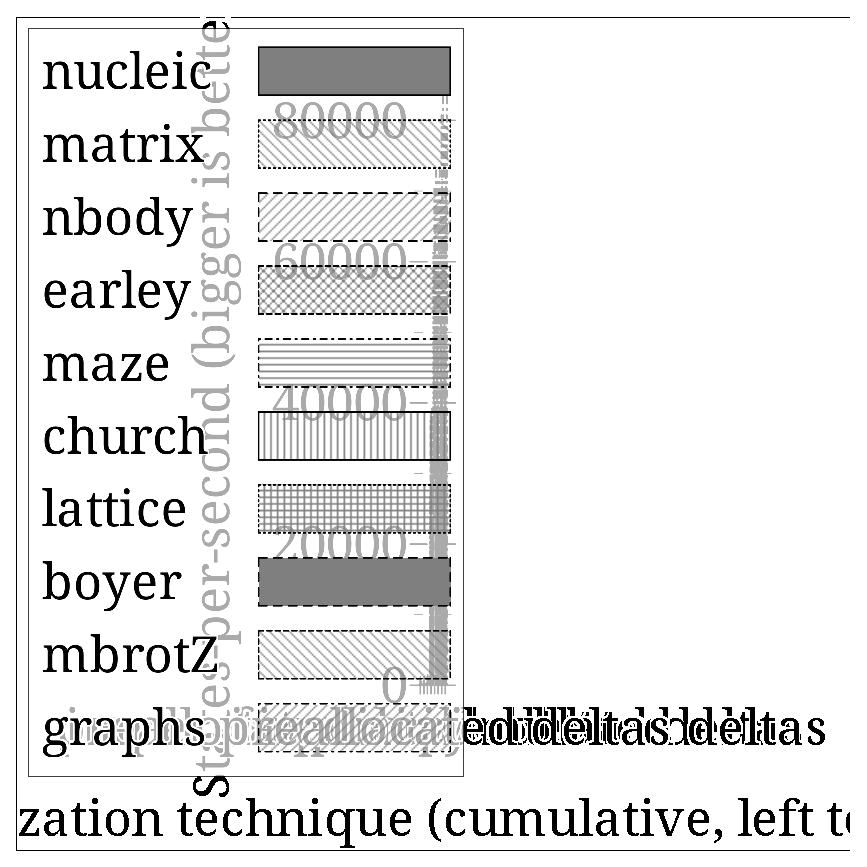
\includegraphics[width=3.2in]{state-per-sec.ps}
\end{center}
\end{figure}

\begin{figure}
\begin{center}
\includegraphics[width=3.2in]{peak-mem.ps}
\end{center}
\end{figure}

\paragraph{Comparison with other flow analysis implementations}

[Computes results more like Earl, et al.'s 0CFA, which times out on
  the Church numeral benchmark and so even though it offers a fair
  point of comparison, a more thorough evaluation is likely to
  uninformative as the other benchmarks are highly likely to timeout
  as well (and it would require significant effort to extend their
  implementation with the features needed to analyze our benchmark
  suite).  That implementation is evaluated against much smaller
  benchmarks: the largest program consists of 63 \emph{subexpressions}
  and times out after 30 minutes.]

Vardoulakis and Shivers evaluate their CFA2
analyzer~\cite{dvanhorn:Vardoulakis2011CFA2} against a variant of 0CFA
defined in their framework.  [NEED TIMING FOR 0CFA ON CHURCH.]  The
Church example is the largest benchmark Vardoulakis and Shivers
consider.  More work would be required to scale the analyzer to the
set of features required by our benchmarks.

[Should probably talk about mCFA too.]

The only analyzers we were able to find that proved capable of
analyzing the full suite of benchmarks considered here were the Soft
Typing system of Wright [CITE] and, in many ways its successor, the
Polymorphic splitting system of Wright and
Jagannathan~\cite{dvanhorn:wright-jagannathan-toplas98}.\footnote{This
  is not a coincidence; these papers set a high standard for
  evaluation, which we consciously aimed to approach.  Many of our
  benchmarks are drawn from these papers.}  Unfortunately, these
analyses compute an inherently different and uncomparable form of
analysis.  Consequently, we have omitted a complete comparison with
these implementations,.  The AAM approach provides more precision in
terms of temporal-ordering of program states, which comes at a cost
that can be avoided in constraint-based approaches.  Consequently
implementation techniques cannot be ``ported'' between these two
approaches.  However, our optimized implementation is within an order
of magnitude of the performance of Wright and Jaganathan's analyzer.
Although we would like to improve this to be more competitive, the
optimized AAM approach still has many strengths to recommend it in
terms of precision, ease of implementation and verification, and rapid
design.




\section{Related work}
\label{sec:related}

\paragraph{Abstracting Abstract Machines}

This work clearly closely follows Van Horn and Might's original papers
on abstracting abstract
machines~\cite{dvanhorn:VanHorn2011Abstracting,dvanhorn:VanHorn2012Systematic},
which in turn is one piece of the large body of research on flow
analysis for higher-order languages (see
Midtgaard~\cite{dvanhorn:Midtgaard2011Controlflow} for a thorough
survey).  The AAM approach sits at the confluence of two major lines
of research: (1) the study of abstract
machines~\cite{dvanhorn:landin-64} and their systematic
construction~\cite{dvanhorn:reynolds-hosc98}, and (2) the theory of
abstract interpretation
\cite{dvanhorn:Cousot:1977:AI,dvanhorn:Cousot:1979:Galois}.


\paragraph{Frameworks for flow analysis of higher-order programs}

Besides the original AAM work, the analysis most similar to that
presented in section~\ref{sec:aam} is the infinitary control-flow
analysis of Nielson and Nielson~\cite{dvanhorn:nielson-nielson-popl97}
and the unified treatment of flow analysis by Jagannathan and
Weeks~\cite{dvanhorn:jagannathan-weeks-popl95}.  Both are
parameterized in such a way that in the limit, the analysis is
equivalent to an interpreter for the language, just as is the case
here.  What is different is that both give a constraint-based
formulation of the abstract semantics rather than a finite machine
model.

\paragraph{Abstract compilation}

Boucher and Feeley \cite{dvanhorn:Boucher1996Abstract} introduced the
idea of \emph{abstract compilation}, which used closure generation
\cite{dvanhorn:Feeley1987Using} to improve the performance of control
flow analysis.  We have adapted the closure generation technique from
composition evaluators to abstract machines and applied it to similar
effect.

\paragraph{Constraint-based program analysis for higher-order languages}

Constraint-based program analyses
(e.g.~\cite{dvanhorn:nielson-nielson-popl97,dvanhorn:wright-jagannathan-toplas98,dvanhorn:Meunier2006Modular})
typically compute sets of abstract values for each program point.
These values approximate the values arising at run-time for each
program point.  Value sets are computed as the least solution to a set
of constraints (either inclusion or equality constraints).  The
constraints must be designed and proved as a sound approximation of
the semantics.  Efficient implementations of these kinds of analyses
often take the form of worklist-based graph algorithms for constraint
solving, and are thus quite different from the interpreter
implementation.  The approach thus requires effort in constraint
system design and implementation, and the resulting system require
verification effort to prove the constraint system is sound and that
the implementation is correct.

This effort increases substantially as the complexity of the analyzed
language increases.  Both the work of maintaining the concrete
semantics and constraint system (and the relations between them) must
be scaled simultaneously.  However, constraint systems, which have
been extensively studied in their own right, enjoy efficient
implementation techniques and can be expressed in declarative logic
languages that are heavily
optimized~\cite{dvanhorn:bravenboer-smaragdakis-oopsla09}.
Consequently, constraint-based analyses can be computed quickly.  For
example, Jagannathan and Wright's polymorphic splitting
implementation~\cite{dvanhorn:wright-jagannathan-toplas98} analyses
the church numeral example of figure~\ref{fig:church} in 7
milliseconds, about 25 times faster than the fastest implementation
considered here.  These analyses compute very different things (as
detailed in section~\ref{sec:accept}), so the performance comparison
is not apples-to-apples.  We view the primary contribution of this
work as a systematic path that eases the design, verification, and
implementation of analyses using the abstracting abstract machine
approach to within a factor of performant constraint-based analyses.

\section{Conclusion}
\label{sec:conclusion}

Abstract machines are not only a good model for rapid analysis
development, they also can be systematically developed into efficient
algorithms.

%% \acks Sam Tobin-Hochstadt for encouragement and feedback -- he was
%% the first to prompt us to look into how make effective
%% implementations of the AAM approach.

%% Vincent St Amour for feedback on early drafts.
%% Greg Morrisset and Matthias Felleisen for discussions.

%% NSF, DARPA

\paragraph{Acknowledgments}

We thank Suresh Jagannathan for providing source code to the
polymorphic splitting
analyzer~\cite{dvanhorn:wright-jagannathan-toplas98} and Ilya Sergey
for the introspective pushdown
analyzer~\cite{dvanhorn:Earl2012Introspective}.

\balance
\bibliographystyle{plain}
\bibliography{local,bibliography}

% \appendix
\section{Relation to Uniform \(k\)-CFA (A Case Against Acceptability)}
\label{sec:accept}

\cite{dvanhorn:nielson-nielson-popl97} \cite{dvanhorn:Neilson:1999}

This machine's allocation strategy mimics the Uniform k-CFA analysis
in Principles of Program Analysis, which is defined in terms of
``$\delta$ contours.''  However, because the machine represetation makes
context explicit via continuations, we can calculate these contours
rather than thread them throught the evaluator.  In other words, we
can use the CESK* machine without modification to obtain Uniform k-CFA
by way of a simple allocation strategy.  (In this way, it's a
simplification of the presentation in JFP.)

NNH uses a coinductive acceptability relation to specify Uniform
k-CFA:

\[
   C,R \models^{ce}_\delta E
\]

The cache and global environment form a finite store-like structure
holding bindings and return values.  The contour environment ce maps
variables to locations in R which contains their bindings, just as the
environment of the CESK* machine does.  The current contour delta is a
string of application labels describing the enclosing context under
which this term is being analyzed (or evaluated).  If you view the
acceptability relation as a big-step evalator, the
$(\widehat C,\widehat\rho)$ component should be seen as a global
store ce is the environment mapping variables to their locations.

Starting form the initial configuration for a program and iterating
the machine transition relation until reaching a fixpoint of reachable
states will \emph{underestimate} the acceptability relation of Uniform
k-CFA.  You can recover acceptability by feeding this store back into
the initial configuration and iterating again.  Repeating this process
until a complete run of the program reaches no new states will be the
least solution that is acceptable.

HOWEVER.  Why should we care about acceptability?  What this
machine computes is safe.  In other words, it computes a more
precise characterization of the run-time behavior of a program.  In
doing is so, it actually saves work (as can be seen above).

An Example:

\begin{alltt}
 (let ((id (\(\lambda\) (x) x)))
   (begin (id 1) (id 2)))
\end{alltt}

Under Uniform 0-CFA, we would have:
\[
   [{\tt x} \mapsto \{{\tt 1}, {\tt 2}\}] \in \widehat\rho
\]

in the least solution to $\models$.  This says that, when run, 'x' is
bound to 1 or 2.

Under the machine semantics using a 0CFA allocation policy, the trace
semantics of the machine show that x is bound to 1, and that at some
later point, x becomes bound to 1 or 2.  Moreover, the machine would
show that (id 1) evaluates to 1 and only 1, while Uniform 0CFA must
give that (id 1) is either 1 or 2 to be acceptable.  We don't see any
value in these kinds of false flows that are due to the global and
timeless aspects of C,R which acceptability requires the heap to be
both finite and unchanging over the course of abstract
interpretation. (Another view of the difference: the machine abstracts
a program's execution as a \emph{finite state machine} that mimics the
machine interpretation of the program; the aceptability relation of
Uniform \(k\)-CFA abstracts a program's execution as a \emph{finite
  map} that mimics the big-step evaluator: from terms to (sets of)
values.)


\subsection{Another problem with acceptability: Temporal ignorance}

The small-step approach to static analysis brings subtle yet important temporal
richness not found in classical analyses for higher-order programs.
%
Classical analyses (ultimately) compute judgments on program terms and
contexts, e.g., at expression $e$, value $x$ may have value $v$.
%
The judgments do not relate the order in which expressions and context may be
evaluated in a program, e.g., a classical analysis has nothing to say with
regard to question like, ``Do we always evaluate $e_1$ before $e_2$?'' or ``Is
it always the case that a file handle is opened, read and then closed in that
order?''

Small-step analyses, by their nature, encode the temporal relationships between
abstract states.
%
It is sensible to make temporal queries of a small-step analysis.
%
Of course, this does not come for free: respecting temporal order imposes an
order in which states and terms may be evaluated \emph{during} the analysis.
%
Classical analyses can (and do) evaluate expressions in any order, or in some
cases, even in parallel~\cite{might:Prabhu:2010:EigenCFA}.
%
Relaxing that restriction on order affords additional optimizations that we
have \emph{not} performed.

We avoid sacrificing order not simply because we are interested in the
questions it allows us to ask, but because considering temporal order actually
improves the precision of the analysis itself.



\section{Pushdown Analysis}

It is straightforward to instantiate a \emph{pushdown} abstraction by
bounding only the variable binding portion of the heap, but using a
unique allocation strategy for continuations.  Such a strategy
abstracts a program's execution as a \emph{pushdown automata}
that mimics the machine interpretation.  This strategy therefore
models the abstract stack in a true stack like fashion and always
properly matches function calls with their return.

Although such analyses can be formulated straightforwardly in the
abstract machine approach, it is not clear all of the techniques of
this paper can be applied to similar effect in the pushdown context.
The main problem is calculation of an analysis can no longer be
computed as the fixed point of the machine transition relation.
Although there are several implementations (CFA2,ICFP'12), they
operate at speeds roughly on par with our starting point: unoptimized
store widened
machines. \cite{dvanhorn:Earl2012Introspective,dvanhorn:Vardoulakis2011CFA2}

\section{Proof: laziness is precision-preserving}
Given widened machine configurations, we can show that lazy
non-determinism is precision-preserving in the cases that application
positions are store-allocated and not. We first show the latter since
it uses less cluttered transition rules. The high level is that the
``fan-out'' of non-determinism is collapsed back in the store (in the
store-allocated applications case) or delayed a single step by
laziness that would have happened in a step of strictness.

Details of lazy machine given as a diff from the strict machine. \\
State space of $lazy-\widehat{CESK}^*_t$ varies just in
$\mathit{Value}$ (storable values do not change):
\begin{align*}
\mval \in \mathit{Value} &::= z \mid b \mid o \mid \saddr{\maddr} \\
\end{align*}

We define a relation between strict and lazy machines that illustrates
the quotient that the lazy states embody.

\newcommand{\vapprx}[3]{#1 \cong_{#2} #3}
\newcommand{\kapprx}[3]{#1 \cong_{#2} #3}
\newcommand{\lapprx}[3]{#1 \approx_{#2} #3}
\newcommand{\apprx}[3]{#1 \sim_{#2} #3}
\newcommand{\capprx}[2]{#1 \sim #2}

\begin{mathpar}
\inferrule{\mval' \in force(\msto, \mval)}
          {\vapprx{\mval}{\msto}{\mval'}} \quad
\inferrule{\ans{\mval} \in cs}{\lapprx{\ans{\mval}}{\msto}{cs}} \quad
\inferrule{\ev{\mexp, \menv, \mkont, \mcntr} \in cs}
          {\lapprx{\ev{\mexp, \menv,\mkont, \mcntr}}{\msto}{cs}} \\
\inferrule{\co{\mkont, \mval'} \in cs \\
           \vapprx{\mval}{\msto}{\mval'}}
          {\lapprx{\co{\mkont, \mval}}{\msto}{cs}} \quad
\inferrule{\ap{\mval_0, \mval_1, \mkont} \in cs \\
           \vapprx{\mval_1}{\msto}{\mval_1'}}
          {\lapprx{\ap{\mval_0, \mval_1', \mkont}}{\msto}{cs}} \\
\inferrule{\ev{\mexp, \menv, \mkont} \in lcs}
          {\apprx{\ev{\mexp, \menv,\mkont}}{\msto}{lcs}} \quad
\inferrule{\ans{\mval} \in lcs \\
           \vapprx{\mval}{\msto}{\mval'}}
          {\apprx{\ans{\mval'}}{\msto}{lcs}} \\
\inferrule{\co{\mkont, \mval} \in lcs \\
           \vapprx{\mval}{\msto}{\mval'}}
          {\apprx{\co{\mkont, \mval'}}{\msto}{lcs}} \quad
\inferrule{\ap{\mval_0, \mval_1, \mkont} \in lcs \\
           \vapprx{\mval_1}{\msto}{\mval_1'}}
          {\apprx{\ap{\mval_0, \mval_1', \mkont}}{\msto}{lcs}} \\
\inferrule{\forall lc \in lcs, \lapprx{lc}{\msto}{cs} \\
           \forall c \in cs, \apprx{c}{\msto}{lcs}}
          {\capprx{(lcs, \msto)}{(cs, \msto)}}
\end{mathpar}

We also need metafunctions for adding and removing a store component
from states. These are straightforwardly defined, so just name them
$wn$ and $nw$ respectively.
%% c2vc(<e^l r k d>,s) = <e^l r s k d>
%% c2vc(<v k d>,s) = <v s k d>
%% vc2c(<e^l r s k d>) = <e^l r k d>
%% vc2c(<v s k d>) = <v k d>

The property we show is that all states stay related through
reduction. The main difficulty is in showing the resulting stores are
in fact equal. We do this by showing each lazy reduction corresponds
to a set of strict reductions, for which the union of their output
stores equal the lazy store. Also for strict equality, every strict
reduction corresponds to a lazy reduction (immediate from the relation).

\begin{lemma}[Partition step]
$\forall lc, lcs', cs, \msto, \msto'.$
 if  $\capprx{(\{lc\},\msto)}{(cs,\msto)}$
 and $\forall lc' \in lcs'. wn(lc,\msto) \machstep wn(lc', \msto')$ then
 $\exists cs'. \forall c \in cs. \exists c' \in cs', \msto^c$
 such that $wn(c,\msto) \machstep wn(c', \msto^c)$
 and       $\msto' = \bigcup\limits_{c \in cs}{\msto^c}$
 and       $\capprx{(lcs',\msto')}{(cs',\msto')}$.
\end{lemma}
\begin{proof}
Let $lc' \in lcs'$ be arbitrary.
By cases on $wn(lc,\msto) \machstep wn(lc', \msto')$:
\begin{itemize}
\item{Case $\ev{\svar{\mvar}, \menv, \mkont, \msto} \machstep \co{\mkont,
    \saddr{\menv(\mvar)}, \msto}$: \\ By definition of $\machstep$,
  $wn(lc,\msto)$ steps strictly to each of $cs' = \{\co{\mval, \mkont} \mid \mval \in \msto(\menv(\mvar))\}$.  By definition of
  $\capprx{}{}$, $cs = \{lc\}$. The stores are the same, and by
  definition of $\lapprx{}{\msto}{}$, $\lapprx{lc'}{\msto}{cs'}$.}
\item{Case $\ev{\slit{\mlit}, \menv, \msto, \mkont, \msto} \machstep
            \co{\mkont, \mlit, \msto}$: \\
      Immeditate.}
\item{Case $\ev{\slam{\mvar}{\mexp}, \menv, \mkont, \msto} \machstep
            \co{\mkont, \clos{\mvar, \mexp, \menv}, \msto}$: \\
      Immediate}
\item{Case $\ev[^\mcntr]{\sapp[^\mlab]{\mexp_0}{\mexp_1}, \menv, \mkont, \msto} \machstep
            \ev[^\mcntr]{\mexp_0, \menv, \msto', \kar[^\mcntr_\mlab]{\mexp_1, \menv, \maddr}, \msto'}$: \\
      Where $\maddr, \msto' = \mathit{push}_\mlab^\mcntr(\msto,\mkont)$ \\
      Immediate.}
\item{Case $\ev[^\mcntr]{\sif[^\mlab]{\mexp_0}{\mexp_1}{\mexp_2}, \menv, \mkont, \msto} \machstep
            \ev[^\mcntr]{\mexp_0, \menv, \msto', \kif[^\mcntr]{\mexp_1, \mexp_2, \menv, \maddr}, \msto'}$: \\
      Where $\maddr, \msto' = \mathit{push}_\mlab^\mcntr(\msto,\mkont)$ \\
      Immediate.}
\item{Case $\co{\kmt, \mval, \msto} \machstep \ans{\msto, \mval'}$: \\
      Where $\mval' \in force(\msto, \mval)$ \\
      By definition of $\capprx{}{}$, $cs = \{\co{\kmt, \mval'} \mid \mval \in force(\msto, \mval)\}$.
      By definition of $\machstep$, $wn(lc,\msto)$ steps strictly to
      each of $cs' = \{\ans{\mval}\}$. The stores are the same.
      By definition of $\lapprx{}{\msto}{}$, $\forall lc' \in lcs'. \lapprx{lc'}{\msto}{cs'}$.
      By definition of $\apprx{}{\msto}{}$, $\forall c' \in cs'. \apprx{c'}{\msto}{lcs'}$.
      Thus $\capprx{(lcs',\msto)}{(cs',\msto)}$.}
\item{Case $\co{\kar[^\mcntr_\mlab]{\mexp, \menv, \maddr}, \mval, \msto} \machstep
            \ev[^\mcntr]{\mexp, \menv, \kfn[^\mcntr_\mlab]{\mval',\maddr}, \msto}$: \\
      Where $v' \in force(\msto, \mval)$. \\
      By definition of $\apprx{}{\msto}{}$,
        $cs = \{\co{\kar[^\mcntr_\mlab]{\mexp, \menv, \maddr}, \mval'} \mid \mval \in force(\msto, \mval)\}$.
      By definition of $\machstep, \lapprx{}{\msto}{}$,
        $cs' = \{\ev[^\mcntr]{\mexp, \menv, \kfn[^\mcntr_\mlab]{\mval',\maddr}}
            \mid \co{\kar[^\mcntr_\mlab]{\mexp, \menv, \maddr}, \mval'} \in cs\}$.
      The stores are the same, and the previous imply $\capprx{(lcs',\msto)}{(cs',\msto)}$.}
\item{Case $\co{\kfn[^\mcntr_\mlab]{\mvalx{u}, \maddr}, \mval, \msto} \machstep
            \ap{\mvalx{u}, \mval, \mkont, \msto}$: \\
      Where $\mkont \in \msto(\maddr)$. \\
      Immediate.}
\item{Case $\co{\kif[^\mcntr]{\mexp_0, \mexp_1, \menv, \maddr}, \mval, \msto} \machstep
            \ev{\mexp_0, \menv, \mkont, \msto}$: \\
      Where $\mkont \in \msto(\maddr)$. \\
      By definition of $\machstep$, $\strue \in force(\msto, \mval)$, thus by definition of
      $\capprx{}{}$, the strict machine takes the same step.}
\item{Case $\co{\kif[^\mcntr]{\mexp_0, \mexp_1, \menv, \maddr}, \mval, \msto} \machstep
            \ev{\mexp_1, \menv, \mkont, \msto}$: \\
      Where $\mkont \in \msto(\maddr)$. \\
      By definition of $\machstep$, $\sfalse \in force(\msto, \mval)$, thus by definition of
      $\capprx{}{}$, the strict machine takes the same step.}
\item{Case $\ap[^\mcntr_\mlab]{\clos{\mvar, \mexp, \menv}, \mval, \mkont,\msto} \machstep
            \ev[^{\mcntr'}]{\mexp, \menv', \mkont, \msto'}$: \\
      Where $\menv', \msto', \mcntr' = \mathit{bind}^\mcntr_\mlab(\menv, \msto, \mvar, \mval)$
      By definition of $\apprx{}{\msto}{}$,
        $cs = \{\ap[^\mcntr_\mlab]{\clos{\mvar, \mexp, \menv}, \mval', \mkont} \mid
                \mval' \in force(\msto, \mval)\}$.
      Thus $cs' = \{\ev[^{\mcntr'}]{\mexp, \menv', \mkont}\}$ (clearly $\lapprx{lc'}{\msto'}{cs'}$)  and
      for all $c \in cs$, $wn(c,\msto) \machstep wn(c',\msto\sqcup[\mvar\mcntr' \mapsto \{c.\mval\}])$.
      Thus the union of these stores is equal to $\msto'$.}
\item{Case $\ap[^\mcntr_\mlab]{\mop, \mval, \mkont,\msto} \machstep
            \co{\mval'', \mkont, \msto}$: \\
      Where $\mval' \in force(\msto, \mval)$
        and $\mval'' \in\interpdelta(\mop,\mval')$. \\
      By definition of $\capprx{}{}$ and $\interpdelta$,
        $cs = \{\ap[^\mcntr_\mlab]{\mop, \mvalx{u}, \mkont} \mid
                \mvalx{u} \in force(\msto, \mval),
                \mval'' \in\interpdelta(\mop,\mvalx{u})\}$.
      Thus the strict machine takes the same step.}
\end{itemize}
\end{proof}


\begin{theorem}[Laziness preserves precision]
$\forall lcs,cs,lcs',\msto,\msto'$ if $\capprx{(lcs, \msto)}{(cs,\msto)}$
  and $(lcs,\msto) \machstep (lcs',\msto')$ then there exists $cs'$
  such that $(cs,\msto) \machstep (cs',\msto')$
\end{theorem}
\begin{proof}
By definition of $\machstep$,
$lcs' = \{lc' \mid \exists \msto^{lc}. wn(lc,\msto) \machstep wn(lc', \msto^{lc}), lc \in lcs\}$
For each $lc \in lcs$ let $\hat{c}^{lc} \subseteq cs$ be the
smallest set such that $\lapprx{lc}{\msto}{\hat{c}^{lc}}$. \\ By the
previous lemma, there exists a $\hat{c}^{lc}{}'$ such that $\capprx{(\{lc' \mid wn(lc,\msto) \machstep
  wn(lc', \msto^{lc})\}, \msto^{lc})}{(\hat{c}',\msto^{lc})}$. Let
$cs' = \bigcup\limits_{lc \in lcs}{\hat{c}^{lc}{}'}$ and $\msto' = \bigcup\limits_{lc \in lcs}{\msto^{lc}}$.
Since each step individually is related, the union is related: $\capprx{lcs'}{\msto'}{cs'}$.
By definition of $\machstep$, $(cs, \msto) \machstep (cs', \msto')$ and $(lcs, \msto) \machstep (lcs', \msto')$.
\end{proof}

%% --Eval
%% <x r s k d> --> <v s k d> where v in s(r(x))  [VAR]
%% <(e0^l0 e1^l1)^{l,lf,la} r s k d> --> <e0^l0 r s\sqcup[ld |-> {k}] ar^{l,lf,la}(e1^l1 r ld) d> [APP]
%% <(lambda x e) r s k d> --> <clos(x e r) s k d> [CLOS]
%% --Continue
%% <v s ar^{l,lf,la}(e^le r a) d> --> <e^le r s\sqcup[lfd |-> {v}] fn^{l,la}(lfd, a)> [CO]
%% --Apply
%% <v s fn^{l,la}(fa, ka) d> --> <e^fl r[x |-> xd'] s'[xd' |-> s'(lad)] k d'> [AP]
%%   where clos(x e^fl r) in s(fa)
%%         k in s(ka)
%%         s' = s\sqcup[lad |-> {v}]
%%         d' = truncate(ld, K)

%% This extra binding corresponds directly to the intermediate
%% bindings introduced by ANF.
%% Matt's ANF analyses likely have all the flavours of our "laziness" technique, but this is how we get our chocolate with our peanut butter as Olin would say.

%% Compare this to lazyCESK^*t:
%% v ::= clos(x e r) | addr(a)
%% Clos ::= clos(x e r)
%% s : a -> P(Clos)
%% others the same

%% force(s, addr(a)) = s(a)
%% force(s, clos(x e r)) = {clos(x e r)}

%% --Eval
%% <x r s k d> --> <addr(r(x)) s k d>
%% others the same
%% --Continue
%% <v s ar^{l,lf,la}(e^le r a) d> --> <e^le r s\sqcup[lfd |-> force(s,v)] fn^{l,la}(lfd, a)>
%% --Apply
%% <v s fn^{l,la}(fa, ka) d> --> <e^fl r[x |-> xd'] s'[xd' |-> s'(lad)] k d'>
%%   where clos(x e^fl r) in s(fa)
%%         k in s(ka)
%%         s' = s\sqcup[lad |-> force(s, v)]
%%         d' = truncate(ld, K)
%% The same globalizing stuff applies.

%% Let us relate the state spaces of the two abstract machines for the lambda calculus in the following way

%% Then we can show that if lazyconf ~ conf and lazyconf ==> lazyconf' then there exists a conf' such that conf ==> conf' and lazyconf' ~ conf'
%% Let lc in lazyconf.cs be arbitrary (call lazyconf.s, s)
%% By cases on lc:
%% <x r k d>:
%% Premises:
%% <x r k d> in conf.cs
%% Thus:
%% Since
%% <x r s k d> -->lazy   <addr(r(x)) s k d>
%% <x r s k d> -->strict <v s k d> where v in s(r(x))
%% By definition of force, v in force(s, addr(r(x)))
%% Thus the first rule of ~_s applies and the second rule of l~_s applies.

%% <(lambda x e) r k d>:
%% Trivial

%% <(e0^l0 e1^l1)^{l,lf,la} r k d>:
%% Premises:
%% <(e0^l0 e1^l1)^{l,lf,la} r k d> in conf.cs
%% Thus:
%% <(e0^l0 e1^l1)^{l,lf,la} r s k d> -->lazy   <e0^l0 r s\sqcup[ld |-> {k}] ar^{l,lf,la}(e1^l1 r ld) d>
%% <(e0^l0 e1^l1)^{l,lf,la} r s k d> -->strict <e0^l0 r s\sqcup[ld |-> {k}] ar^{l,lf,la}(e1^l1 r ld) d>

%% Stores are same in this case.

%% <v ar^{l,lf,la}(e^le r a) d>:
%% Premises:
%% For all v' in force(s, v),
%%   <v' ar^{l,lf,la}(e^le r a) d> in conf.cs
%% Thus:
%% <v ar^{l,lf,la}(e^le r ka) d> -->lazy   <e^le r s\sqcup[lfd |-> force(s, v)] fn^{l,la}(lfd ka) d>
%% for all v' in force(s,v),
%% <v' ar^{l,lf,la}(e^le r ka) d> -->strict <e^le r s\sqcup[lfd |-> {v'}] fn^{l,la}(lfd ka) d>
%% Thus the union of all the strict stores will equal the lazy store.

%% <v fn^{l,la}(fa ka) d>:
%% Premises:
%% For all v' in force(s,v),
%%   <v' fn^{l,la}(fa ka) d> in conf.cs
%% Thus
%% <v fn^{l,la}(fa ka) d> -->lazy <e^fl r[x |-> xd'] s'\sqcup[xd' |-> s'(lad)] k d'>
%% where k in s(ka)
%%       clos(x e^fl r) in s(fa)
%%       d' = truncate(ld, K)
%%       s' = s\sqcup[lad |-> force(s,v)]
%% For all v' in force(s,v),
%% <v' fn^{l,la}(fa ka) d> -->strict <e^fl r[x |-> xd'] s'\sqcup[xd' |-> s'(lad)] k d'>
%% where k in s(ka)
%%       clos(x e^fl r) in s(fa)
%%       d' = truncate(ld, K)
%%       s' = s\sqcup[lad |-> {v'}]

%% Thus the union of all the strict stores will equal the lazy store.




\end{document}
